\documentclass{article}
\usepackage{lscape}
\usepackage[utf8]{inputenc}
\usepackage{tikz}
\usetikzlibrary{shapes.geometric}
\graphicspath{ {images/} }
\usepackage{imakeidx}
\usepackage{amsmath}
\usepackage{amsthm}
\usepackage{framed}
\usepackage{subcaption} 
\usepackage{lscape}
\usepackage[style=authoryear,sorting=nyt]{biblatex}
\usepackage[margin=1in]{geometry}
\linespread{1.5}
\usepackage{longtable}
\usepackage{tocloft}
\usepackage[portuguese]{babel}
\addbibresource{bib.bib}
\newtheorem{mydef}{Definição}
\usepackage{hyperref}

\hypersetup{
    colorlinks=true,
    linkcolor=blue,
    filecolor=blue,      
    urlcolor=blue,
    citecolor=gray,
}
 
\title{Análise Prospectiva dos Efeitos Heterogêneos de uma Liberalização Comercial sobre o Mercado de Trabalho}
\author{Carlos Góes \thanks{Secretaria Especial de Assuntos Estratégicos (SAE/PR) e Universidade da Califórnia \textemdash San Diego.} \and Alexandre Messa \thanks{Instituto de Pesquisa Econômica Aplicada (IPEA).} \and Eduardo Leoni \thanks{Secretaria Especial de Assuntos Estratégicos (SAE/PR).}}
\date{Setembro de 2017 \\ Versão Preliminar}

\begin{document}

\maketitle

\begin{abstract}
Recentemente, a literatura sobre comércio internacional passou a incorporar, em análises de liberalizações prospectivas, fricções no mercado de trabalho. Paralelamente, em  análises retrospectivas, passou-se a explorar os efeitos heterogêneos de choques comerciais em distintas regiões de um mesmo país. Este trabalho combina essas duas inovações e desenvolve um método de estimação de efeitos regionais heterogêneos da liberalização sobre o mercado de trabalho numa análise prospectiva, mesmo na ausência de matrizes regionais de insumo-produto. Após a estimação de elasticidades heterogêneas quanto a resposta laboral de cada região-setor a choques setoriais agregados, utiliza-se um modelo de equilíbrio geral computável, com fricções laborais, para calibrar a dimensão dos choques agregados e estimar efeitos regionais. \\
Palavras-Chave: comércio internacional, liberalização comercial, efeitos regionais, integração do mercado doméstico, modelo de equilíbrio geral computável. \\
Códigos JEL: F11, F13, F15, F16, F17, C33.
\end{abstract}

\newpage

\renewcommand{\cftsecleader}{\cftdotfill{\cftdotsep}}
\tableofcontents
\addtocontents{toc}{~\hfill\textbf{Página}\par}


\newpage

\listoffigures
\addtocontents{lof}{~\hfill\textbf{Página}\par}

\newpage


\section{Introdução}

O fato de o comércio permitir ganhos agregados de bem-estar é relativamente pouco controverso na literatura econômica. Com mais trocas comerciais, firmas e indivíduos têm a possibilidade de se especializar naquelas atividades em que são mais produtivos e ter acesso a outros bens e serviços, intercambiando os excedentes que não consomem. Ademais, firmas têm acesso a máquinas e equipamentos mais baratos e podem, assim, reduzir seus custos operacionais e, ao aumentar sua produtividade e competitividade, pagar salários maiores a seus trabalhadores ao mesmo tempo em que ofertam produtos a preços unitários menores no mercado. Por isso, há evidências de que, após uma liberalização comercial, as taxas de crescimento econômico tendem a subir (ver, p.ex., \textcite{wacziarg}, \textcite{frankelromer} e \textcite{edwards}). 

Em grande medida, os modelos simulacionais de comércio internacional refletem essa conclusão empírica. Recentemente, contudo, avanços na literatura de comércio internacional exploram, com mais detalhes, os efeitos distributivos e regionais de liberalizações comerciais, fricções nos mercados de trabalho e bens e a heterogeneidade na produtividade e remuneração de fatores entre distintos países e distintas indústrias de um mesmo país.

\textcite{EatonKortum} incluíram na modelagem do comércio internacional, desde um ponto de vista ricardiano, diferenças de produtividade e remuneração de fatores entre países e entre distintas indústrias de cada um dos países. Nessa perspectiva, o comércio entre os países se originaria a partir das diferenças de produtividade entre eles, fazendo com que a sensibilidade dos fluxos comerciais a variações de tarifas dependa da dispersão dessa produtividade. \textcite{CaliendoParro} extendem o trabalho de \textcite{EatonKortum} para múltiplos setores, modelando a interação entre eles por meio das matrizes de insumo-produto de cada país inserido na análise.

Inicialmente, os modelos de comércio presumiam perfeita mobilidade intersetorial de trabalhadores, o que faria com que a força de trabalho fosse rapidamente realocada para os setores mais eficientes e os efeitos sobre os salários fossem pequenos. \textcite{artuc} romperam com tal presunção e estimaram empiricamente os custos de mobilidade intersetorial para os Estados Unidos, concluindo que os efeitos salariais de um choque de preços relativos é mais alto do que o presumido anteriormente.

Finalmente, \textcite{caliendo} combinaram os modelos de heterogeneidade internacional e intersetorial em produtividade delineados em \textcite{CaliendoParro} e \textcite{EatonKortum} com as fricções de mobilidade laboral entre setores introduzidas por \textcite{artuc}, permitindo a investigação prospectiva da dinâmica do mercado de trabalho na presença de ampla heterogeneidade de produtividade. Nesse sentido, os agentes representativos analisam custos de transição entre setores e os salários futuros esperados nos múltiplos setores da economia e maximizam sua utilidade decidindo para qual setor mudar, sendo que a nova remuneração dos fatores de produção após um choque de preços relativos é determinada pelas diferenças internacionais de produtividade setorial.

Paralelamente, em análises empíricas recentes, passou-se a  explorar os efeitos regionalmente heterogêneos de choques comerciais em distintas regiões de um mesmo país, particularmente sobre o mercado de trabalho. \textcite{AutorDornHanson}, por exemplo, demonstraram que as regiões dos Estados Unidos que estão mais expostas à competição de manufaturas chinesas tiveram perdas relativas de emprego e salários \textemdash e que os mercados laborais locais têm ajustes muito lentos.

Boa parte da literatura sobre os efeitos heterogêneos de choques comerciais sobre os mercados de trabalho regionais explora a liberalização comercial brasileira ocorrida nos anos 1990. As reduções tarifárias daquele período levaram a ganhos agregados de produtividade na indústria, que se deram tanto diretamente, pela pressão de competição externa que acompanha a maior disponibilidade de bens importados \parencite{rossi}; quanto indiretamente, por meio da redução dos custos de máquinas, equipamentos e insumos para firmas brasileiras \parencite{lisboa}. A despeito de efeitos setoriais, os efeitos nacionalmente agregados de longo prazo sobre o mercado de trabalho foram pequenos. 

Contudo, \textcite{dixcarneiro}, \textcite{dixkovak} e  \textcite{kovak}  demonstraram que as regiões mais expostas aos choques comerciais tiveram uma perda relativa de emprego formal e salários em relação às outras regiões do país. Houve, portanto, ampla heterogeneidade quanto aos efeitos regionais.

Isso ocorreu essencialmente por dois motivos. Primeiramente, os distintos setores da economia estão espacialmente geograficamente concentrados, de modo que o tamanho do choque de preços relativos é diferente para cada região do país. Ademais, os ajustes no mercado de trabalho tem se mostrado muito mais lentos do que se tinha como consenso da literatura sobre o efeito de choques de comércio. A demora para o pleno ajuste do mercado de trabalho parece decorrer da pouca integração dos mercados de trabalho e inflexibilidade das leis trabalhistas, levando os trabalhadores a se deslocarem do setor formal para o informal nas regiões mais afetadas pela liberalização. Tal resultado é consistente com outras análises, que demonstram que o mercado doméstico brasileiro é relativamente pouco integrado \parencite{goes}.

Este trabalho combina essas duas inovações e desenvolve um método de estimação de efeitos regionais heterogêneos da liberalização sobre o mercado de trabalho numa análise prospectiva, mesmo na ausência de matrizes regionais de insumo-produto.

Partiu-se de um Modelo de Equilíbrio Geral Computável (EGC) que utiliza matrizes de insumo-produto para 57 setores econômicos do Brasil e 27 outras unidades (25 países, a União Europeia e um agregado para o resto do mundo). O modelo é baseado em \textcite{caliendo}, incorporando, portanto, variações intersetoriais e internacionais de produtividade e fricções no mercado de trabalho.

Posteriormente, foram utilizados dados da Relação Anual de Informações Sociais (RAIS) entre 2002 e 2015 para agregar níveis de emprego correspondentes a cada um dos 57 setores incluídos no modelo de EGC tanto no nível nacional quanto no nível estadual. Para cada díade estado-setor foi estimada uma elasticidade que denota a resposta percentual esperada de um setor em um estado específico à variação de 1\% no agregado nacional para aquele setor.

Ao total, foram estimadas 1.539 elasticidades que são específicas para cada estado e setor. As elasticidades são heterogêneas, de modo que é possível que, historicamente, num mesmo setor, o emprego tenha sido muito responsivo a mudanças nacionais no emprego em um estado específico e pouco responsivo em outro estado.

Ao fim, estimou-se o efeito esperado para cada setor em cada microrregião ao combinar-se o tamanho do choque nacional para cada setor com a elasticidade específica para cada estado-setor (que foi aplicada homogeneamente para todas as microrregiões de um estado). Ao agregar-se os efeitos esperados de cada um dos 57 setores para cada uma das microrregiões, foi possível estimar o efeito líquido esperado sobre o emprego formal para cada microrregião.

Os resultados indicam relativa heterogeneidade nos efeitos regionais sobre o mercado de trabalho. De forma consistente com as conclusões retrospectivas de \textcite{dixkovak}, observa-se que, prospectivamente, as regiões que enfrentariam um maior choque de preços relativos no caso de uma liberalização comercial também sofreriam impactos relativamente maiores sobre o mercado de trabalho. 

Este trabalho está organizando em quarto seções. Inicialmente, descreve-se o Modelo de Equilíbrio Geral Computável, utilizado para realizar simulações num nível nacional. Posteriormente, é descrita a metodologia de estimação de elasticidades heterogêneas que permitiu chegar a resultados regionalmente heterogêneos mesmo partindo-se de um modelo agregado. Em seguida, apresentam-se os resultados prospectivos nacionalmente agregados (advindos do modelo EGC) e os efeitos heterogêneos regionais sobre o mercado de trabalho. Finalmente, discute-se quais as implicações dos resultados prospectivos para o desenho futuras de políticas públicas e conclui-se revisitando alguns dos principais pontos do trabalho e explicando como o método aqui desenvolvido pode ser expandido para outros países.

\section{Modelo de Equilíbrio Geral Computável}

O modelo utilizado neste trabalho, baseado em \textcite{caliendo}, compreende dois tipos agentes: indivíduos e firmas. Os indivíduos detêm os fatores de produção e consomem bens finais produzidos pelas firmas. As firmas produzem bens finais e intermediários, e, para tal, necessitam empregar e remunerar os fatores de produção detidos pelos indivíduos.

A produção de cada bem utiliza uma variedade de insumos arbitrariamente grande, a partir de uma função de produção com elasticidade de substituição constante (CES, na sigla em inglês) e equivalente a $\sigma$. Por meio de uma função de produção Cobb-Douglas, cada insumo é produzido utilizando-se fatores de produção (capital, trabalho, etc.), além dos bens $1,\ldots,J$ como seus próprios insumos. Cada um desses componentes é empregado na produção a uma proporção equivalente a $\lambda^l, \lambda^{1,j}, \hdots, \lambda^{J,j}$ (com $\lambda^l$ e $\sum_{i=1}^J \lambda^{i,1} = 1$).

Tais dinâmicas se dão em $J$ setores econômicos diferentes de $N$ distintos países. A distribuição da demanda é específica a cada país e os indivíduos no país $n$ consomem frações  $\alpha^n_1 , \hdots , \alpha^n_J$ dos produtos $1 , \hdots , J$, com valores normalizados de tal modo que $\sum_{j=1}^J \alpha^n_j = 1$.

Firmas em cada setor $j$ podem produzir muitos bens intermediários e um bem final a partir de uma função de produção com elasticidade de substituição constante e equivalente a $\sigma$. Por meio de uma função Cobb-Douglas, cada insumo é produzido utilizando-se fatores de produção ($\gamma ^ l$), além dos produtos $1, \hdots , J$ como seus próprios insumos $(\gamma ^ {1,k}, \hdots , \gamma ^ {J,k})$, com valores normalizados de tal modo que $\gamma ^ l + \sum_{j=1}^J \gamma ^{j,k} = 1$.


A função de produção de cada firma contém um termo multiplicativo $z_1^j$, específico a cada setor e país, que representa os respectivos níveis de eficiência. Em outras palavras, cada setor em cada país detém um nível de eficiência $z_n^j$, determinado a partir de uma distribuição de probabilidade Fréchet. Esta distribuição depende de dois parâmetros, $T_n$ e $\theta ^j$ (formalmente, $Pr(z_n^j \leq z) = e^{-T_n z^{ -\theta^j } }$), que determinam, respectivamente, as devidas vantagens absoluta e comparativa. Por um lado, o parâmetro $T_n$ varia conforme o país em questão, e representa o estado-da-arte de sua tecnologia. Mais precisamente, quanto maior for o valor de $T_n$, maior a eficiência esperada de cada setor do país em questão – por isso, esse parâmetro pode ser interpretado como uma medida de vantagem absoluta.

Por outro lado, o parâmetro $\theta^j$ varia ao longo dos setores (sendo porém fixo ao longo dos países para cada setor): quanto menor for o valor de $\theta^j$, maior tende a ser a dispersão de produtividade entre os países na produção do setor $j$. Dessa forma, ele costuma ser interpretado como uma medida de potencial de surgimento de vantagens comparativas em cada setor.
O nível de eficiência $z_n^j$ determina então, para cada país e setor, as respectivas vantagens comparativas em relação à produção de cada insumo m. Sendo $M$ um número arbitrariamente grande (formalmente, $M \to \infty$), %FIX: O que é M?
pela lei dos grandes números cada país proverá, à produção do bem $j$, uma proporção dos insumos $m$ equivalente à proporção de insumos nos quais ele detém uma posição de vantagem comparativa.

\subsection{Mercado de Trabalho}

A parte do mercado de trabalho do modelo de \textcite{caliendo} é baseada em \textcite{artuc}. Supõe-se que determinado país $n$ seja dotado de uma certa quantidade de trabalhadores que ofertam uma unidade de trabalho e recebem um salário $w_t^{nj}$, em que $t$ representa o ano em questão, e $j$, o setor de atividade econômica no qual o trabalhador está empregado. Porém, cada trabalhador dessa economia pode também estar desempregado ($j=0$), caso em que ele recebe uma quantia equivalente a $w_t^{n0}$, correspondendo a um seguro-desemprego ou à chamada produção doméstica.

Para o trabalhador migrar de setor, ele necessita incorrer em um custo $C^{(nj,k)}$, em que $j$ representa o setor de origem, e $k$, o de destino. Assim, esse custo de transição varia de acordo tanto com o setor no qual o trabalhador está correntemente empregado, quanto com o setor para o qual ele deseja migrar. Além disso, caso o trabalhador se encontre no setor $j$ ao final do período $t$, ele coleta um benefício idiossincrático $\epsilon_t^{nj}$. Tais benefícios são i.i.d. ao longo dos indivíduos, setores e períodos, com média zero, e seguem uma distribuição de Valor Extremo do Tipo-I (ou distribuição Gumbel).

Assim, o trabalhador, a cada período, observa as condições correntes e futuras do mercado de trabalho, de forma a optar pelo setor que maximiza sua utilidade ao longo da vida. Formalmente, este problema pode ser sintetizado como:

\begin{equation}
    u_t^{nj} = \ln \frac{w_t^{nj}}{P_t^n} + \max_{k} \{ \beta E[u_{t+1}^{nk} ] - C^{nj,k} + \nu \epsilon_t^k \} 
\end{equation}

em que $u_t^{nj}$ representa a utilidade ao longo da vida de um trabalhador do setor $j$ no ano $t$; o parâmetro $\nu$, um termo que multiplica escalarmente a variância dos choques idiossincráticos; $\beta$, a taxa de desconto dos indivíduos dessa economia; e $P_t^n$, o índice de preços ideal do país $n$ no ano $t$. Em conformidade com \textcite{caliendo}, supõe-se ainda $w_t^{n0}=P_t^n b^n$, de tal forma que o benefício que o trabalhador recebe ao estar desempregado permanece constante ao longo do período. 

A partir do contexto desenvolvido até o momento, e definindo $V_t^{nj}=E[u_t^{nj} ]$ (ou seja, $V_t^{nj}$ representa a utilidade média do trabalhador do setor j no ano t), pode-se mostrar que 

\begin{equation}
    V_t^{nj} = \ln \frac{w_t^{nj}}{P_t^n} + \nu \ln \{ \sum_{k=0}^J \exp (\beta V_{t+1}^{nj} - C^{nj,k} ) ^ {1/\nu}  \}
\end{equation}

Pela equação acima, o valor de estar alocado em determinado setor depende, por um lado, do salário corrente, e, por outro, do valor de opção de migrar para os demais setores.

Em seguida, defina $\mu_t^{nj,k}$ como o percentual de trabalhadores do setor $j$ que migram para o setor $k$ no ano $t$. Então, o problema de maximização do trabalhador leva a dois resultados importantes. Em primeiro lugar, tem-se

\begin{equation}
    \mu_t^{nj,k} = \frac{ \exp (\beta V_t^{nj} - C^{nj,k}) ^ {1/ \nu} }{ \sum_{h=0}^J \exp (\beta V_t^{nh} - C^{nj,k}) ^ {1/ \nu} }
\end{equation}

Pelo resultado acima, após descontado o custo de transição, quanto maior for a utilidade esperada no setor $k$, maior será o percentual de trabalhadores que migrarão para este setor. A partir da equação acima, a alocação de trabalhadores ao longo do tempo será dada pela dinâmica abaixo:

\begin{equation}
    L_{t+1}^{nj} = \sum_{k=0}^J \mu_t^{nk,j}L_t^{nk}
\end{equation}


em que $L_t^{nj}$ representa o número de trabalhadores no setor $j$, no ano $t$.

\subsection{Definição de equilíbrio}

Para a devida caracterização do equilíbrio na economia introduzida acima, é necessário introduzir algumas formalizações. Dessa forma, seja:

\begin{itemize}
    \item $c_t^{nj}$, o custo unitário de fabricação do bem $j$ no país $n$, no ano $t$;
	\item $w_t^{nj}$, o salário do trabalhador do setor $j$ no país $n$, no ano $t$;
	\item $r_t^{nj}$, a remuneração do capital do setor $j$ no país $n$, no ano $t$;
	\item $\xi^{nj}$, o percentual do capital no valor adicionado do setor $j$ no país $n$;
	\item $P_t^{nj}$, o preço do bem $j$ no país $n$, no ano $t$;
	\item $\tau_t^{ni,j}$, a tarifa de importação aplicada pelo país $n$ sobre o bem $j$ oriundo do país $i$ (acrescido da unidade), no ano $t$;
	\item $d_t^{ni,j}$, o custo de transporte do bem $j$, do país $i$ ao país $n$, no ano $t$;
	\item $\pi_t^{ni,j}$, a proporção de bens do setor $j$ importada pelo país $n$ a partir do país $i$, no ano $t$;
	\item $X_t^{nj}$, o total gasto em bens do setor $j$ no país $n$, no ano $t$;
	\item $L_t^{nj}$, o número de pessoal ocupado do setor $j$ no país $n$, no ano $t$;
	\item $H_t^{nj}$, o estoque de capital do setor $j$ no país $n$, no ano $t$;
	\item $I_t^n$, a absorção total do país $n$, no ano $t$.
	\item $S_t^n$, o saldo comercial do país $n$, no ano $t$.
\end{itemize}


A respeito das definições acima, é importante ainda apontar que a absorção $I_t^n$ é resultado da soma dos salários, da remuneração do capital, da receita com o imposto de importação e do déficit comercial. Então, o equilíbrio da economia é caracterizado pela Definição ($D1$) abaixo.


\begin{mydef}\label{def_eq}
Dados ($L_0,S,T,d,C,H$), um equilíbrio competitivo sequencial sob uma estrutura tarifária $\tau$ consiste em uma sequência $\{ L,\mu,V,w \}_{t=1}^{\infty}$ que satisfaz (1), (2) e (3), além de, para todo $j$,$n$,$t$, as equações abaixo:

    \begin{eqnarray}
    c_t^{nj} &=& B^{nj} [(r_t^{nj} )^{\xi^{nj} } (w_t^{nj} )^{1-\xi^{nj}} ]^{\gamma^{nj}} \prod_{k=1}^J (P_t^k) ^ {\gamma ^ {nk,j}} \\
    P_t^{nj} &=& A^j [\sum_{i=1}^N T_i^j (c_t^{ij} d_t^{ni,j} \tau_t^{ni,j} )^{-\theta^j } ] ^ {-1 / \theta^j } \\
    \pi_t^{ni,j} &=& \frac{ T_i^j (c_t^{ij} d_t^{ni,j} \tau_t^{ni,j} )^{-\theta^j } }{ \sum_{h=1}^N T_h^j (c_t^{hj} d_t^{nh,j} \tau_t^{nh,j})^{-\theta^j } } \\
    X_t^{nj} &=& \sum_{k=1}^J \gamma_n^{j,k} \sum_{i=1}^N X_t^{ik} \frac{\pi_t^{in,k}}{1+\tau_t^{in,k}} + \alpha_n^j I_t^n \\
    L_t^{nj} &=& \frac{\gamma^{nj} (1-\xi^{nj})}{w_t^{nj}} \sum_{i=1}^N \pi_{t}^{in,j} X_t^{ij} \\
    H_t^{nj} &=& \frac{\gamma^{nj} \xi^{nj}}{r_t^{nj}} \sum_{i=1}^N \pi_t^{in,j} X_t^{ij} 
    \end{eqnarray}

em que $A^j$ representa uma constante intrínseca a cada setor, e $B^{nj}$, uma constante intrínseca a cada setor de cada país.  
\end{mydef}

\subsection{Resultados de choques tarifários}

A \textit{Definição (D1)} introduz a caracterização do equilíbrio a partir de uma estrutura tarifária $\tau$. O passo seguinte é então investigar como esse equilíbrio se altera a partir de uma mudança de $\tau$ para uma nova estrutura tarifária $\tau'$. Essa mudança de equilíbrio é dada pela \textit{Definição (D2)} abaixo.

\begin{mydef}
Defina $Y_{t+1}^{nj}=\exp⁡(V_{t+1}^{nj}-V_t^{nj})$. Então, a partir de uma mudança de estrutura tarifária de $\tau$ para $\tau^{'}$, as condições de equilíbrio devem satisfazer a equação (xx) e as variações relativas:

\begin{eqnarray}
    \label{eq:D2a}
    \hat{c}_n^j &=& [(\hat{w}_t^{nj})^{(1 - \xi^{nj} ) } (\hat{r}_t^{nj} )^{ \xi^{nj} } ]^{\gamma_n^j } \prod_{k=1}^J 
    \hat{P}_t^{nk^ { \gamma_n^{k,j} } }  \\
    \label{eq:D2b}
    \hat{P}_t^{nj} &=& [\sum_{i=1}^N T_i^j (\hat{c}_t^{ij} \hat{\tau}_t^{ni,j})^{-\theta^j}]^{-1 / \theta^j } \\
    \label{eq:D2c}
    \hat{\pi}_t^{ni,j} &=& [\frac{\hat{c}_t^{ij} \hat{\tau}_t^{ni,j}}{\hat{P}_t^{nj}}]^{-\theta^j} \\
    \label{eq:D2d}
    X_{t+1}^{nj} &=& \sum_{k=1}^J \gamma_n^{j,k}  \sum_{i=1}^N X_{t+1}^{ik}   \frac{\pi_{t+1}^{in,k}}{1+\tau_{t+1}^{in,k}} + \alpha_n^j I_{t+1}^n \\
    \label{eq:D2e}
    \sum_{j=1}^J \sum_{i=1}^N X_{t+1}^{ij}  \frac{\pi_{t+1}^{ni,j}}{1+\tau_{t+1}^{ni,j}} + S_{t+1}^n &=& \sum_{j=1}^J \sum_{i=1}^N X_{t+1}^{ij}  \frac{ \pi_{t+1}^{in,j}}{1+\tau_{t+1}^{in,j} } \\
    \label{eq:D2f}
    \mu_{t+1}^{nj,k} &=& \frac{\mu_t^{nj,k} (Y_{t+2}^{nk} )^\beta }{ \sum_{h=0}^J \mu_t^{nj,h} (Y_{t+2}^{nh} )^\beta } \\
    \label{eq:D2g}
    Y_{t+1}^{nj} &=& (\frac{\hat{w}_{t+1}^{nj}}{\hat{P}_{t+1}^n}) \sum_{h=0}^J \mu_t^{nj,h} (Y_{t+2}^{nh})^\beta \\
    \label{eq:D2h}
    \hat{w}_{t+1}^{nj} \hat{L}_{t+1}^{nj} w_t^{nj} L_t^{nj} &=& \gamma^{nj} (1-\xi^{nj}) \sum_{i=1}^N \pi_{t+1}^{in,j} X_{t+1}^{ij}
    \end{eqnarray}
\end{mydef}

As equações acima representam, respectivamente: as alterações nos respectivos custos unitários de produção (\ref{eq:D2a}), nos preços dos produtos (\ref{eq:D2b}) e nas proporções de comércio bilateral (\ref{eq:D2c}); o gasto total no bem $j$ por parte do país $n$ (\ref{eq:D2d}); a balança comercial (\ref{eq:D2e}); as migrações intersetoriais por parte dos trabalhadores (\ref{eq:D2f}); o crescimento da utilidade esperada dos trabalhadores de cada setor (\ref{eq:D2g}); e, finalmente, a condição de market-clearing (\ref{eq:D2h}). Dessa forma, para investigar os resultados a partir de choques nos custos de importação, o procedimento adotado consiste em resolver as equações acima.

\subsection{Calibragem com microdados laborais}

Em primeiro lugar, admita como disponíveis os dados referentes a: fluxos comerciais entre os países para cada bem $j$; o total do valor adicionado de cada setor $j$, em cada país $n$; a produção total de cada setor $j$, em cada país $n$; as matrizes de insumo-produto de cada país $n$, desagregadas conforme os setores $j$; a distribuição inicial de trabalhadores ao longo dos setores, $L_0$; e, finalmente, a migração inicial entre setores, $\mu_{t-1}$. A partir desses dados, obtém-se: 

\begin{itemize}
    \item $\pi_{ni}^j$, como a proporção dada pela própria definição da variável;
    \item $\gamma_n^j$ dados pela proporção do valor agregado do setor $j$ em relação ao valor total de sua produção por parte do país $n$;
    \item $\gamma_n^{j,k}$, dados pelas matrizes de insumo-produto de cada país;
    \item $\alpha_n^j$, dado por $(Q_n^j - S_n^j - \sum_{k=1}^J \gamma_k^{j,n} Q_n^k) / I_n $ , em que $Q_n^j$ representa o produto do setor $j$ no país $n$.
\end{itemize}

As tabelas 1 e 2 descrevem as quantidades de equações e variáveis a serem estimadas.  Assim, para cada período, tem-se um total de $N(6J+2)+N^2 [J+(J+1)^2]$ equações disponíveis para a estimação do mesmo número de variáveis. Como usual em modelos de equilíbrio geral, o trabalho consiste então em determinar o vetor de preços que faça com que os mercados entrem em equilíbrio. No presente modelo, o preço básico da economia é dado pelos salários $w_t^{nj}$. Com isso, o algoritmo consiste em encontrar o vetor $\hat{w}_t^{nj}$ que gera a igualdade no sistema de equações apontado na \textit{Definição (D2)}. \\

\begin{center}
\begin{table}[ht]
\caption{Número de equações a partir das condições de equilíbrio (por período).}
\begin{center}
\begin{tabular}{ll}
\hline 
    \textbf{Condições de equilíbrio} & \textbf{Número de equações}\tabularnewline
\hline 
    $\hat{c}_n^j = [(\hat{w}_t^{nj})^{(1 - \xi^{nj} ) } (\hat{r}_t^{nj} )^{ \xi^{nj} } ]^{\gamma_n^j } \prod_{k=1}^J \hat{P}_t^{nk^ { \gamma_n^{k,j} }}$ & $NJ$ \tabularnewline

    $\hat{P}_t^{nj} = [\sum_{i=1}^N T_i^j (\hat{c}_t^{ij} \hat{\tau}_t^{ni,j})^{-\theta^j}]^{-1 / \theta^j }$ & $NJ$ \tabularnewline
    
    $ \hat{\pi}_t^{ni,j} = [\frac{\hat{c}_t^{ij} \hat{\tau}_t^{ni,j}}{\hat{P}_t^{nj}}]^{-\theta^j}$ & $N^2J$ \tabularnewline
    
    $X_{t+1}^{nj} = \sum_{k=1}^J \gamma_n^{j,k}  \sum_{i=1}^N X_{t+1}^{ik}   \frac{\pi_{t+1}^{in,k}}{1+\tau_{t+1}^{in,k}} + \alpha_n^j I_{t+1}^n$ & $NJ$ \tabularnewline
    
    $\mu_{t+1}^{nj,k} = \frac{\mu_t^{nj,k} (Y_{t+2}^{nk} )^\beta }{ \sum_{h=0}^J \mu_t^{nj,h} (Y_{t+2}^{nh} )^\beta }$ & $N^2(J+1)^2$ \tabularnewline
    
    $Y_{t+1}^{nj} = (\frac{\hat{w}_{t+1}^{nj}}{\hat{P}_{t+1}^n}) \sum_{h=0}^J \mu_t^{nj,h} (Y_{t+2}^{nh})^\beta$ & $N(J+1)$ \tabularnewline
    
    $\hat{w}_{t+1}^{nj} \hat{L}_{t+1}^{nj} w_t^{nj} L_t^{nj} = \gamma^{nj} (1-\xi^{nj}) \sum_{i=1}^N \pi_{t+1}^{in,j} X_{t+1}^{ij}$ & $NJ$ \tabularnewline
    
    $L_{t+1}^{nj} = \sum_{k=0}^J \mu_t^{nk,j} L_t^{nk}$ & $N(J+1)$ \tabularnewline
    
\hline 

    \textbf{Total} & \textbf{$N(6J+2)+N^2 [J+(J+1)^2]$} \tabularnewline
\hline    
\end{tabular}
\end{center}
\end{table}
\end{center}

\begin{center}
\begin{table}[ht]
\caption{Número de variáveis envolvidas nas condições de equilíbrio (por período).}
\begin{center}
\begin{tabular}{ll}
\hline 
    \textbf{Variáveis} & \textbf{Número de variáveis}\tabularnewline
\hline 
    $\hat{w}_t^{nj}$ & $NJ$ \tabularnewline
    
    $\hat{r}_t^{nj}$ & $NJ$ \tabularnewline
    
    $\hat{P}_t^{nj}$ & $NJ$ \tabularnewline
    
    $\hat{\pi}_t^{ni,j}$ & $N^2J$ \tabularnewline
    
    $X_t^{nj}$ & $NJ$ \tabularnewline
    
    $\mu_t^{nj,k}$ & $N^2 (J+1)^2$ \tabularnewline
    
    $Y_t^{nj}$ & $N(J+1)$ \tabularnewline
    
    $L_t^{nj}$ & $N(J+1)$ \tabularnewline
    
\hline 

    \textbf{Total} & \textbf{$N(6J+2)+N^2 [J+(J+1)^2]$} \tabularnewline
\hline    
\end{tabular}
\end{center}
\end{table}
\end{center}

É importante observar que, no presente modelo, as alterações tarifárias exercem efeitos de equilíbrio geral ao longo da economia. No caso, uma redução da tarifa sobre importações do produto do setor $X$ por parte de determinado país tende a ter dois efeitos. Um primeiro efeito é mais imediato, tornando mais barato o consumo final do produto em questão. No entanto, há também um segundo efeito, tornando mais barato o consumo intermediário por parte do setor $Y$ que utiliza o produto do setor $X$ como insumo. Dessa forma, haverá uma redução no custo de produção do setor $Y$ e, consequentemente, uma queda em seus preços domésticos.

Essa queda no preço do produto do setor $Y$ no país em questão exerce, por sua vez, outros dois efeitos. Em primeiro lugar, torna mais barata a importação desse produto por parte de outros países. Em segundo lugar, caso o bem em questão tivesse uma desvantagem de custo e não fosse exportado, pode passar a sê-lo. Com isso, mudanças na estrutura tarifária exercem efeitos tanto sobre a margem intensiva de comércio, quanto sobre a margem extensiva. Em outras palavras, alterações tarifárias, no presente modelo, podem tanto afetar a quantidade importada a partir de antigos parceiros comerciais (margem intensiva), quanto alterar o país que é capaz de fornecer determinado bem a um menor custo (margem extensiva).  

\section{Cálculo de elasticidades e mapeamento regional das variações sobre o emprego}

Para cada díade correspondente a um estado ($s = [1,...,27]'$) e setor um GTAP ($g = [1,...,57]'$), nós calculamos $1.539$ elasticidades que medem a resposta percentual esperada do emprego em cada díade a mudanças nos estoques nacionalmente agregados de emprego em seu respectivo setor GTAP. O modelo base, que controla por características invariáveis no tempo específicas de cada díade, é formalmente especificado da seguinte maneira:

\begin{equation}
    e_{s,g,t} = \phi_{s,g}e_{g,t}^{\#} + c_{s,g} + u_{s,g,t}, \qquad \phi \sim (\mu_\phi,\sigma_\phi^2), \qquad u \sim (0,\sigma_u^2), \quad I(0), \quad iid.
    \label{equation:painel}
\end{equation}

onde $e_{s,g,t}$ é o logaritmo do emprego no setor GTAP $g$ para o estado $s$ no ano $t$; $e_{g,t}^{\#}$ é o logaritmo do emprego agregado nacionalmente para o setor GTAP $g$, definido como $e_{g,t}^{\#} = \sum_{s=1}^{27} e_{s,g,t}$; $c_{s,g}$ são interceptos específicos para cada díade; e $u_{s,g,t}$  são resíduos, tomados como estacionários e distribuídos normalmente. As elasticidades $\phi$, que são os parâmetros de interesse, são heterogêneas para díades diferentes, com primeiro ($\mu_\phi$) e segundo ($\sigma_\phi^2$) momentos existentes e bem definidos.

A estimação de elasticidades heterogêneas é razoável na medida em que é esperado que cada díade estado-setor responda de forma distinta a choques nacionais agregados. Portanto, ao utilizarmos elasticidades heterogêneas, incorporamos mais informação, por meio de maior variabilidade, resultando, assim, em estimações mais precisas nos níveis menos agregados. Conforme demonstrado por \textcite{pesaran}, na análise de séries temporais, quando as dinâmicas são heterogêneas, a estimação de parâmetros homogêneos pode levar a resultados enviesados, sendo preferível a estimação de uma regressão para cada membro do painel.

As elasticidades calculadas, conforme esperado, são relativamente pequenas, concentrando-se quase integralmente no intervalo entre $\pm1,5$ ao redor de $1$. A distribuição de elasticidades aproxima-se a uma distribuição normal centrada na média e com desvio padrão de um (ver Figura \ref{fig:elastic_hist}).

\begin{figure}[ht]
    \centering
    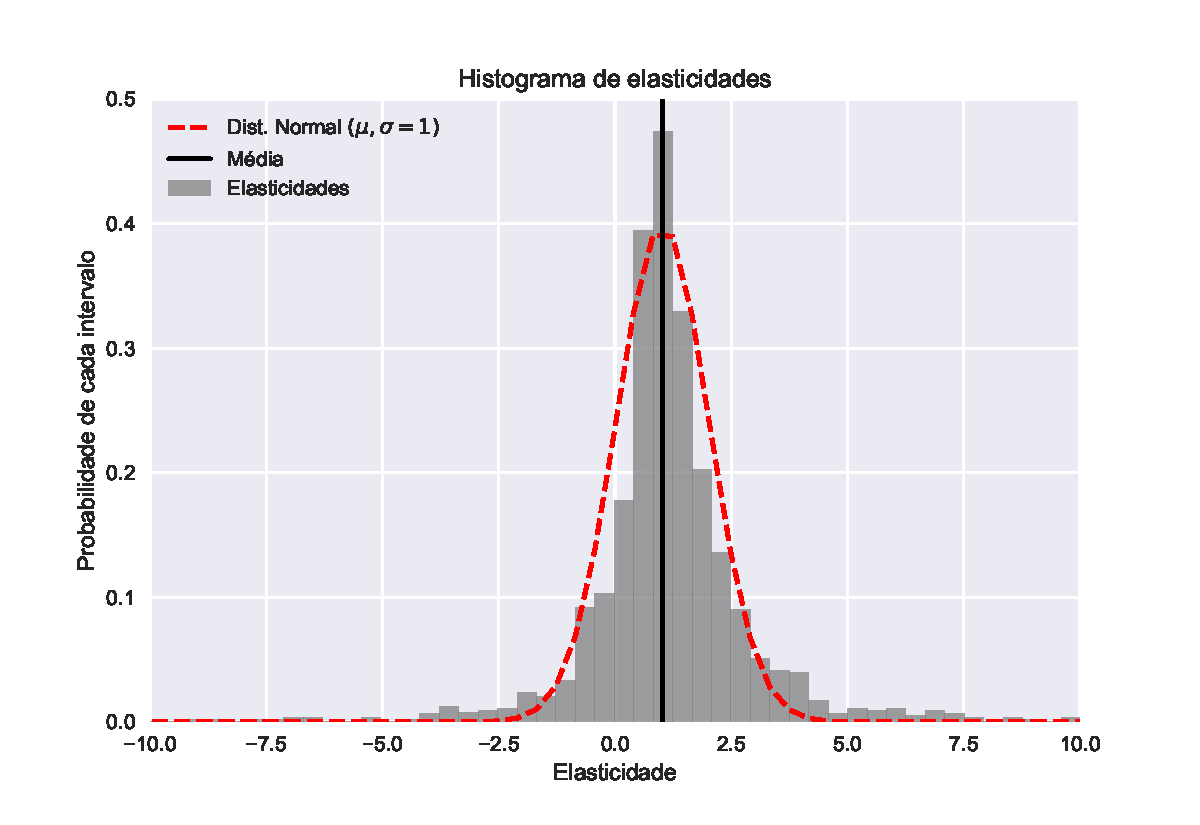
\includegraphics[scale=0.6]{elastic_hist.pdf}
    \caption[Elasticidades locais: histograma]{\textbf{Elasticidades locais: histograma}. Descreve a distribuição probabilística das elasticidades estimadas para cada uma das $1.539$ díades estado-setor.}
    \label{fig:elastic_hist}
\end{figure}

Ademais, as estimativas menos incertas (isto é, aquelas com t-valor mais alto) também concentram-se ao redor de um (ver Figura \ref{fig:elastic_scatter}). Tal resultado é intuitivo: ele denota que os \textit{outliers} estimados tendem a ter erros padrões maiores. Isso é, em larga medida, explicado pelo fato de que, em algumas díades estado-setor, a força de trabalho é muito pequena, restringindo, assim, a série temporal da variável dependente estimada em (\ref{equation:painel}). As díades com maior força de trabalho tendem a ter t-valores maiores \textemdash e, portanto, elasticidades menos incertas (ver Figura \ref{fig:amostra_scatter}).

\newpage 

\begin{figure}[ht]
    \centering
    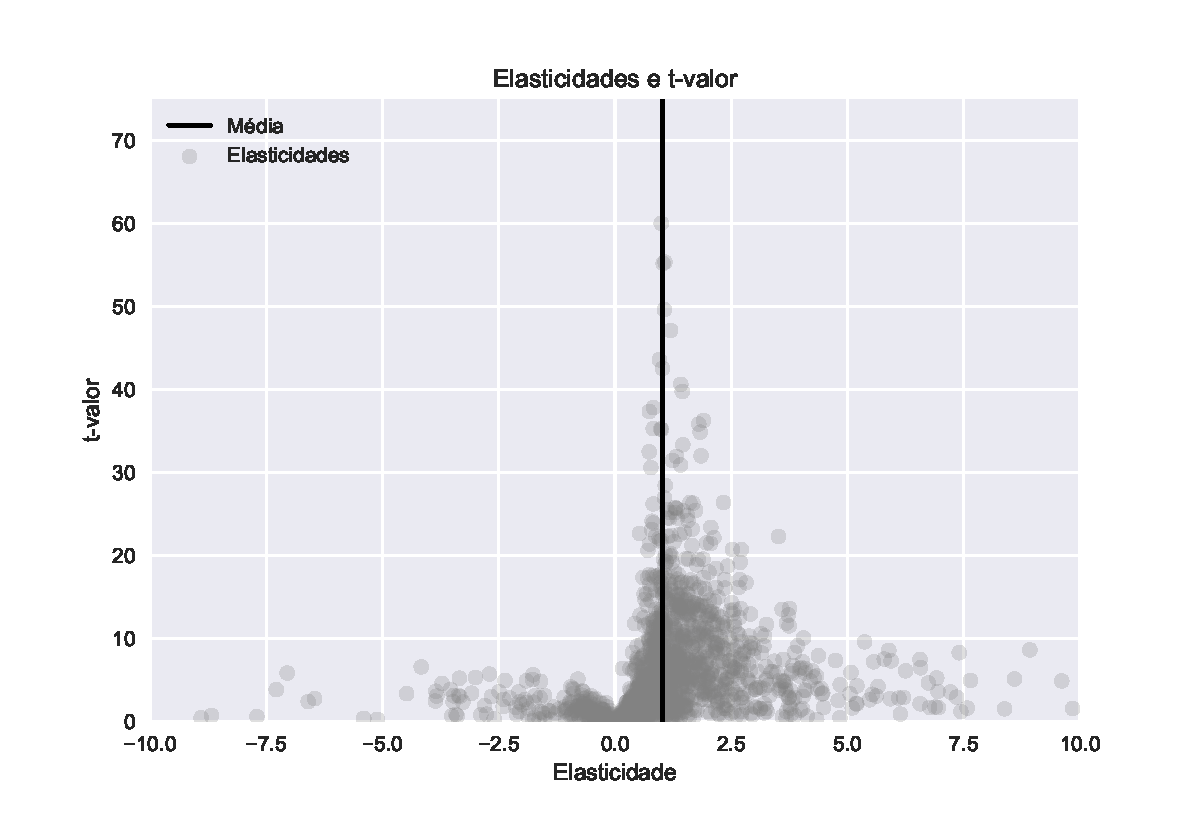
\includegraphics[scale=0.6]{elastic_scatter.pdf}
    \caption[Elasticidades locais: parâmetros e t-valor]{\textbf{Elasticidades locais: parâmetros e t-valor}. Descreve a relação entre elasticidades estimadas para cada uma das $1.539$ díades estado-setor e seu t-valor.}
    \label{fig:elastic_scatter}
\end{figure}


\begin{figure}[ht!]
    \centering
    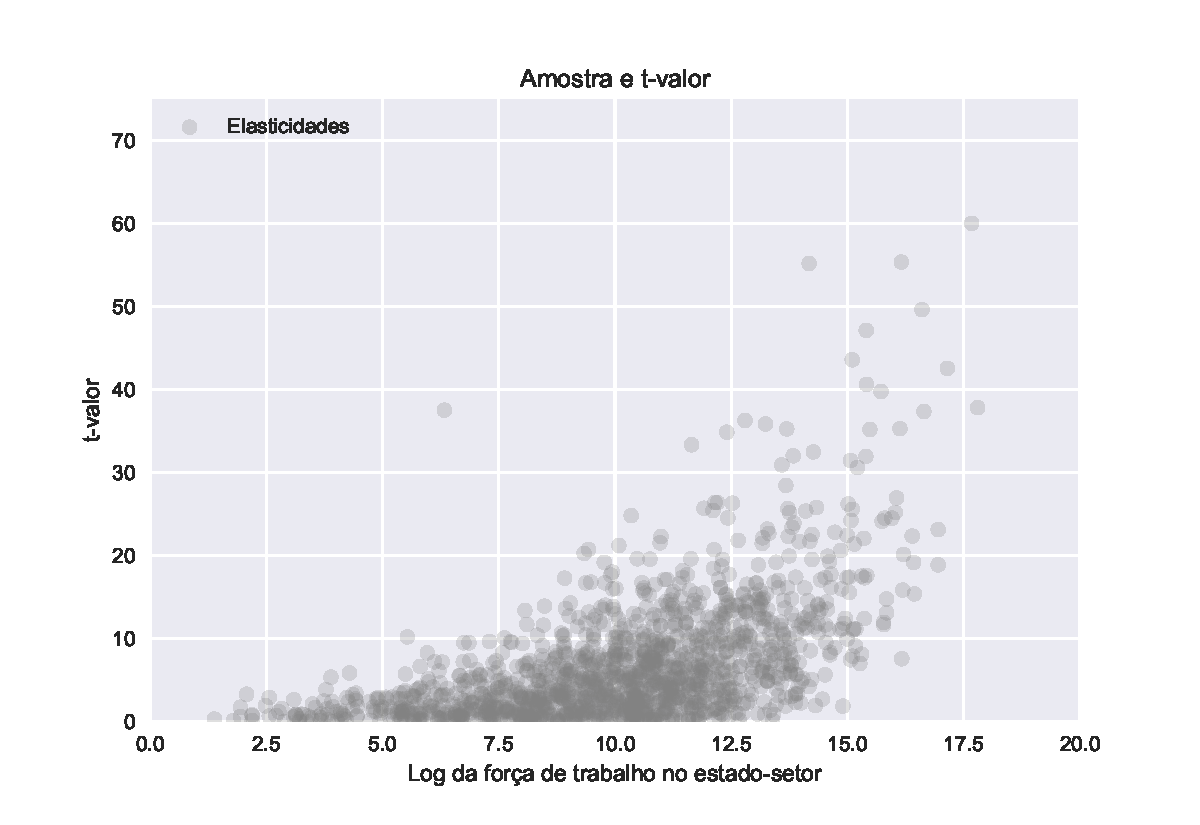
\includegraphics[scale=0.6]{amostra_scatter.pdf}
    \caption[Elasticidades locais: amostra e t-valor]{\textbf{Elasticidades locais: amostra e t-valor}. Descreve a relação entre a força de trabalho em cada uma das $1.539$ díades estado-setor e seu t-valor.}
    \label{fig:amostra_scatter}
\end{figure}

Após calcular as elasticidades, nós as combinamos com os resultados do Modelo de Equilíbrio Geral Computável – isto é, as variações nacionais no emprego, para cada setor GTAP, após um choque tarifário específico, para um horizonte específico. Assumindo que as elasticidades são homogêneas dentro de cada estado, chegamos a variações esperadas no emprego para cada setor GTAP em cada microrregião, após a liberalização:


\begin{equation}
    \Delta e_{m,s,g,t+k}^* = \phi_{m,s,g} \Delta e_{g,t+k}^*, \qquad \phi_{m,s,g} = \phi_{s,g} \forall m  
\end{equation}

em que os asteriscos denotam valores simulados; $t$ denota o ano de liberalização; $k$ representa o horizonte futuro simulado; $\phi_{m,s,g}$ representa a elasticidade específica para cada microrregião e setor; e $\Delta e_{g,t+k}^*$ representa a variação cumulativa no emprego simulada para o setor GTAP g entre o ano de liberalização $t$ e o horizonte de simulação $k$. 

Por fim, calculamos o efeito líquido esperado sobre o emprego para cada microrregião, ao calcular uma média ponderada que incorpora o peso de cada setor GTAP para cada microrregião ($\lambda_{m,s,g}$):

\begin{equation}
    \label{eq:micro_agg}
    \Delta e_{m,s,g,t+k}^* = \sum_{g=1}^{57} \lambda_{m,s,g} \phi_{m,s,g} \Delta e_{g,t+k}^*
\end{equation}

\section{Resultados} 

\subsection{Resultados setoriais agregados nacionalmente} 

Os resultados do modelo de equilíbrio geral computável inclui previsões sobre produção, emprego, salário, preços, importação e exportação de 57 setores diferentes das economias brasileira e dos outros países do mundo. A simulação contempla os efeitos esperados sobre cada variável nos distintos setores da economia \textbf{após a eliminação de todas as tarifas aplicadas pelo governo brasileiro à importação}. Esse é tido como um cenário de referência, vendo os efeitos mais extremados possíveis sobre o mercado de trabalho. O instrumental desenvolvido, contudo, permite traçar vários cenários possíveis, com liberalização de tarifas e barreiras não-tarifárias.

Após uma liberalização comercial, os trabalhadores tendem a sair daqueles setores que são hoje mais protegidos – e menos competitivos – e migrar para aqueles setores mais competitivos. Uma vez que o efeito é primordialmente de migração entre setores, o nível total de emprego se mantém inalterado (mais precisamente, com uma queda esperada no desemprego de 0,015\%).

É importante enfatizar, contudo, que durante todo o período que se segue à liberalização comercial, 75\% dos setores da economia brasileira passam por uma expansão de emprego e, ao final do período de 20 anos, espera-se que apenas três setores da economia brasileira tenham uma redução no emprego setorial maior que 0,5\% (ver Figura \ref{fig:mod_estatico_po}).

Um efeito esperado da maior integração ao mercado internacional é a redução de preços domésticos. Por um lado, a competição de fornecedores internacionais limita a capacidade de empresas nacionais conseguirem aumentar preços por serem as únicas a fornecer determinado produto no mercado doméstico. Por outro lado, como as firmas nacionais passam a ter acesso a insumos e máquinas mais baratas, elas conseguem também produzir a custos unitários menores, aumentando assim sua competitividade.

Essas dinâmicas são capturadas na simulação. No agregado, observa-se uma redução no nível geral de preços de cerca de 5\%, em relação ao cenário sem liberalização. Quando são analisadas as mudanças de preços por setor da economia, há muita variabilidade (ver Figura \ref{fig:mod_estatico_precos}). Alguns setores, que já acompanham preços internacionais (como petróleo) ou que não são comercializáveis internacionalmente (como residências) não têm redução nenhuma nos preços. Já aqueles setores que hoje são muito protegidos, como automóveis, maquinários, couro, têxteis e vestuários, têm uma redução nos preços entre 6\% e 16\%.


Com essa redução nos preços, as firmas menos competitivas tendem a não sobreviver – o que leva os trabalhadores a mudar para outros setores da economia. Os setores mais protegidos originalmente tendem a ter uma redução maior de sua participação na economia nacional (ver Figura \ref{fig:mod_estatico_prod}). Presumivelmente, são setores que não conseguiam produzir a preços similares a seus competidores internacionais e, sendo menos eficientes, tiveram que reduzir sua força de trabalho e produção total.  

É importante notar, contudo, que mesmo os setores que, aparentemente, mais sofrem com o aumento da concorrência internacional passam a ter custos unitários menores e, ao se tornarem mais competitivos, conseguem exportar mais (ver Figura \ref{fig:mod_estatico_exp}, que inclui 42 setores que produzem bens comercializáveis) em relação ao cenário pré-abertura comercial. Com isso, observa-se também nos resultados da simulação a supracitada relação de que mais importações levam a maior competitividade e, como consequência, mais exportações.

Por último, o choque tarifário leva a um reajuste no equilíbrio salarial no mercado de trabalho, com salários caíndo nos setores que se contraem e aumentando nos setores que se expandem. Cerca de 75\% dos setores têm aumento esperado de salários (ver Figura \ref{fig:mod_estatico_sal}). A lógica subjacente dos resultados é que o valor adicionado de cada firma remunera seus fatores de produção. Na medida em que alguns setores produzem menos, o valor adicionado será menor. Com isso, havendo alguma dificuldade para mudança intersetorial, quando a redução percentual da população ocupada naquele setor é menor do que a redução percentual do valor adicionado, os salários tendem a cair. A queda do salário faz com que o trabalhador saia da firma e procure outra, tendendo a levar a alguma recuperação do salário. Ainda assim, espera-se que boa parte do ajuste ao choque comercial ocorra por meio de ajustes salariais.

\newpage
\begin{landscape}
\begin{figure}[htbp!]
    \centering
    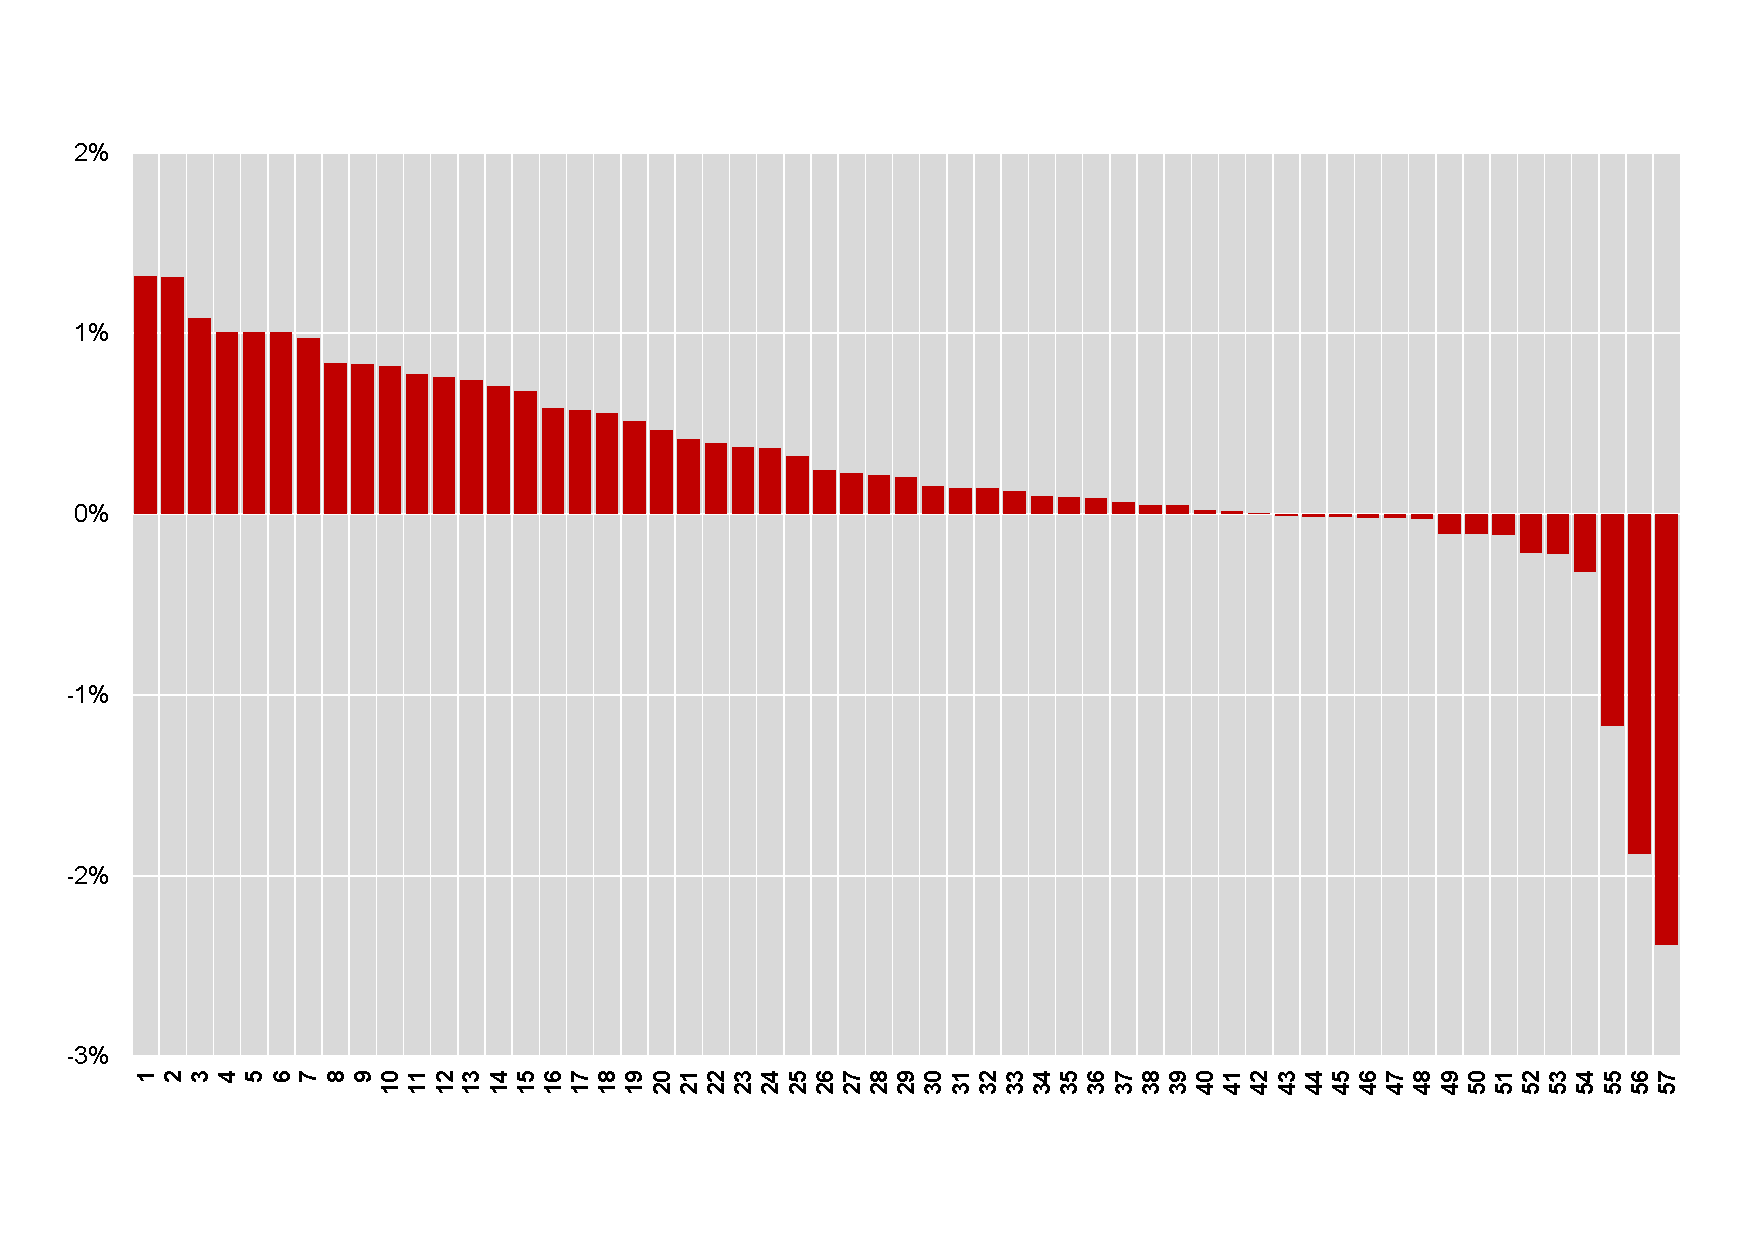
\includegraphics[scale=0.8]{mod_estatico_po.pdf}
    \caption[Modelo CGE: População Ocupada]{\textbf{Modelo CGE: População Ocupada}. Variação percentual cumulativa da população formal ocupada, por setor GTAP, 20 anos após o choque de abertura comercial. \scriptsize{1. Carvão; 2. Outros minérios; 3. Derivados do petróleo; 4. Oleaginosas; 5. Gás; 6. Petróleo; 7. Trigo; 8. Outros grãos; 9. Outras colheitas; 10. Metais não ferrosos; 11. Carne in natura; 12. Outras carnes; 13. Açúcar; 14. Pecuária; 15. Papel; 16. Frutas e vegetais; 17. Cana de açúcar; 18. Outros produtos animais; 19. Fibras vegetais; 20. Óleos vegetais; 21. Distribuição de gás; 22. Arroz in natura; 23. Pescados; 24. Produtos florestais; 25. Outros equip. de transporte; 26. Ferro e aço; 27. Eletricidade; 28. Químicos; 29. Outros alimentos; 30. Outros transportes; 31. Madeira; 32. Transportes aquaviários; 33. Arroz processado; 34. Minerais não-metálicos; 35. Transportes aeroviários; 36. Serviços comerciais; 37. Comunicações; 38. Água; 39. Intermediação financeira; 40. Comércio; 41. Leite; 42. Seguros; 43. Laticínios; 44. Construção; 45. Lã; 46. Recreação; 47. Governo; 48. Residências; 49. Equipamentos eletrônicos; 50. Automóveis e peças; 51. Bebidas e tabaco; 52. Outros maquinários; 53. Outras manufaturas; 54. Produtos de metal; 55. Couro; 56. Têxteis; 57. Vestuário.}}
    \label{fig:mod_estatico_po}
\end{figure}
\end{landscape}

\newpage
\begin{landscape}
\begin{figure}[htbp]
    \centering
    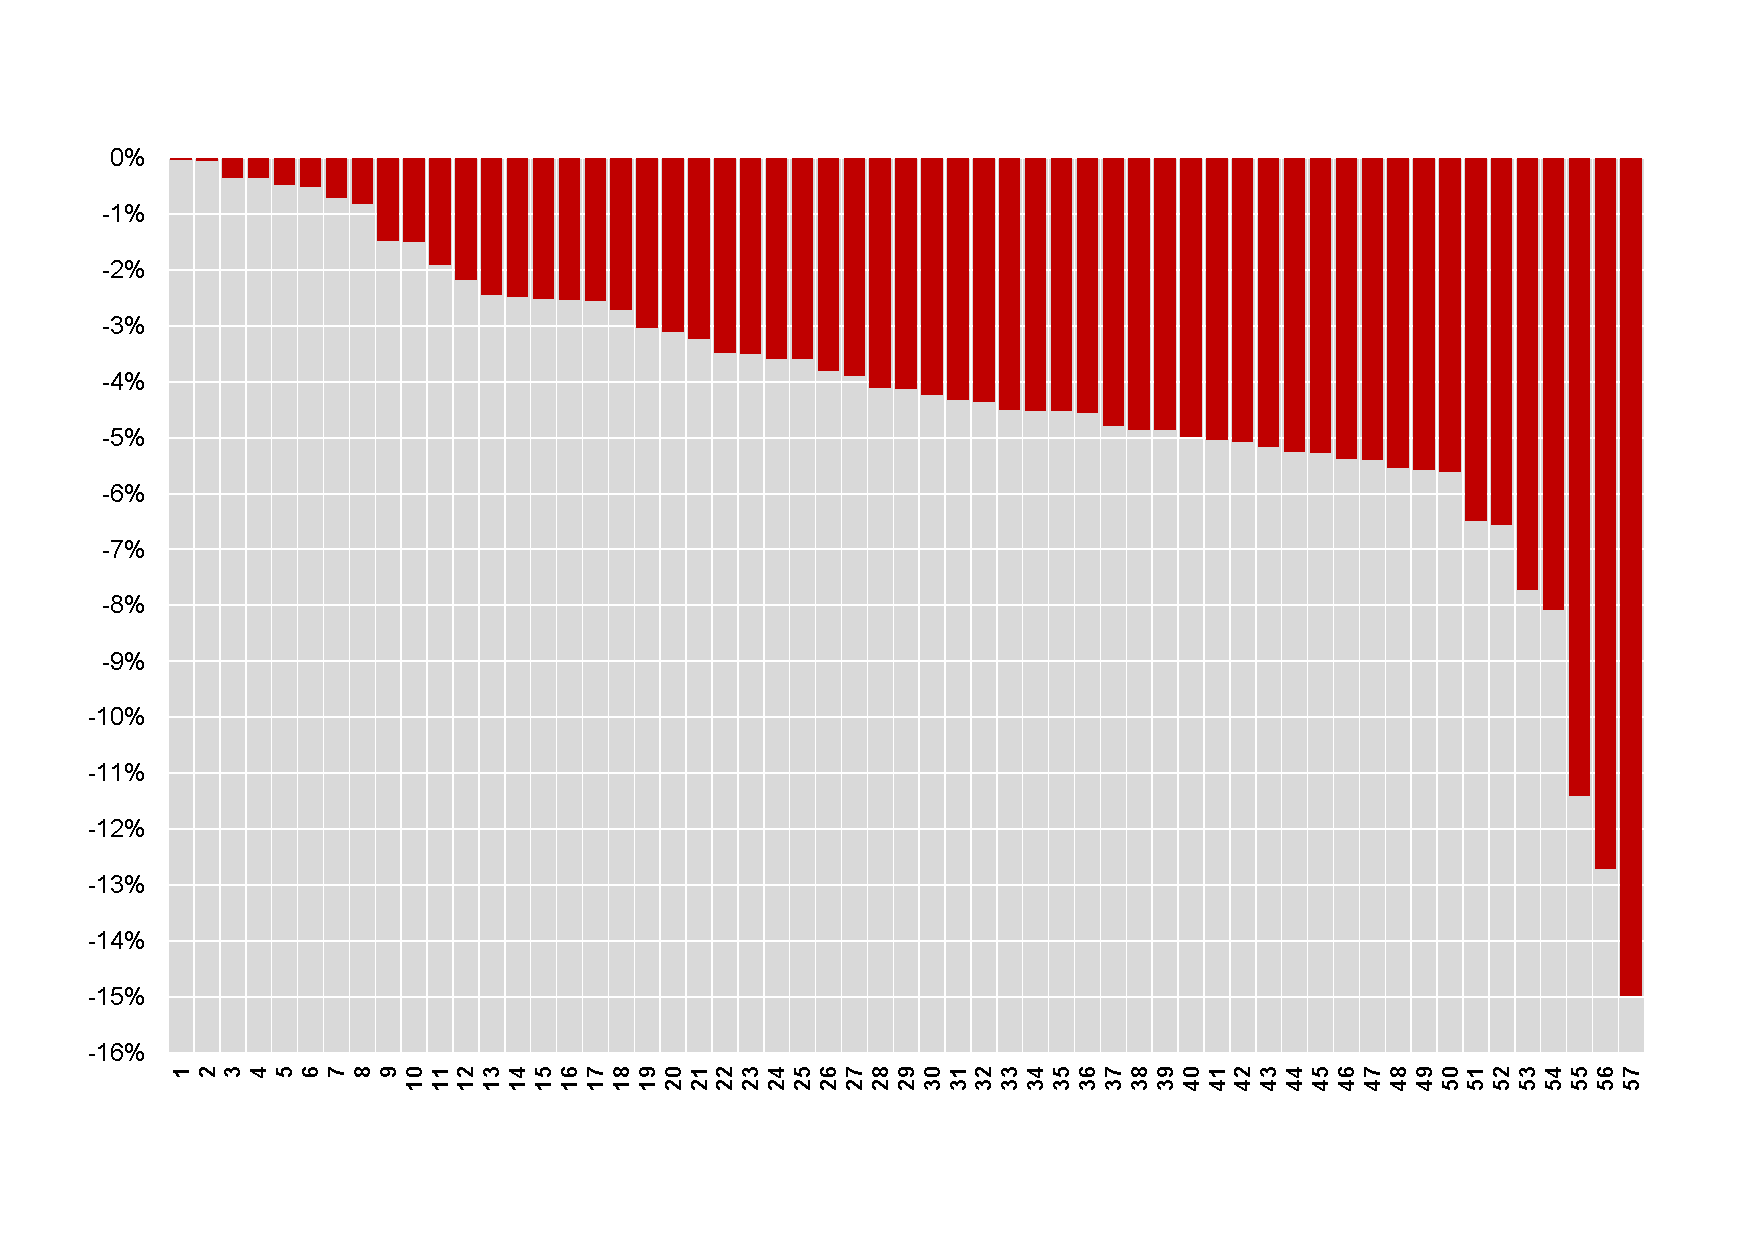
\includegraphics[scale=0.8]{mod_estatico_precos.pdf}
    \caption[Modelo CGE: Preços]{\textbf{Modelo CGE: Preços}. Variação percentual cumulativa dos preços, por setor GTAP, 20 anos após o choque de abertura comercial. \scriptsize{1. Gás; 2. Petróleo; 3. Pescados; 4. Residências; 5. Carvão; 6. Frutas e vegetais; 7. Papel; 8. Arroz in natura; 9. Trigo; 10. Fibras vegetais; 11. Outras colheitas; 12. Outros minérios; 13. Oleaginosas; 14. Arroz processado; 15. Carne in natura; 16. Ferro e aço; 17. Pecuária; 18. Outras carnes; 19. Eletricidade; 20. Produtos florestais; 21. Outros grãos; 22. Madeira; 23. Lã; 24. Cana de açúcar; 25. Açúcar; 26. Outras manufaturas; 27. Transportes aquaviários; 28. Outros transportes; 29. Comércio; 30. Laticínios; 31. Minerais não-metálicos; 32. Leite; 33. Automóveis e peças; 34. Derivados do petróleo; 35. Outros produtos animais; 36. Químicos; 37. Óleos vegetais; 38. Distribuição de gás; 39. Seguros; 40. Transportes aeroviários; 41. Outros alimentos; 42. Comunicações; 43. Construção; 44. Intermediação financeira; 45. Água; 46. Recreação; 47. Serviços comerciais; 48. Governo; 49. Couro; 50. Outros equip. de transporte; 51. Outros maquinários; 52. Metais não ferrosos; 53. Produtos de metal; 54. Equipamentos eletrônicos; 55. Vestuário; 56. Bebidas e tabaco; 57. Têxteis.}}
    \label{fig:mod_estatico_precos}
\end{figure}
\end{landscape}
\newpage

\begin{landscape}
\begin{figure}[htbp]
    \centering
    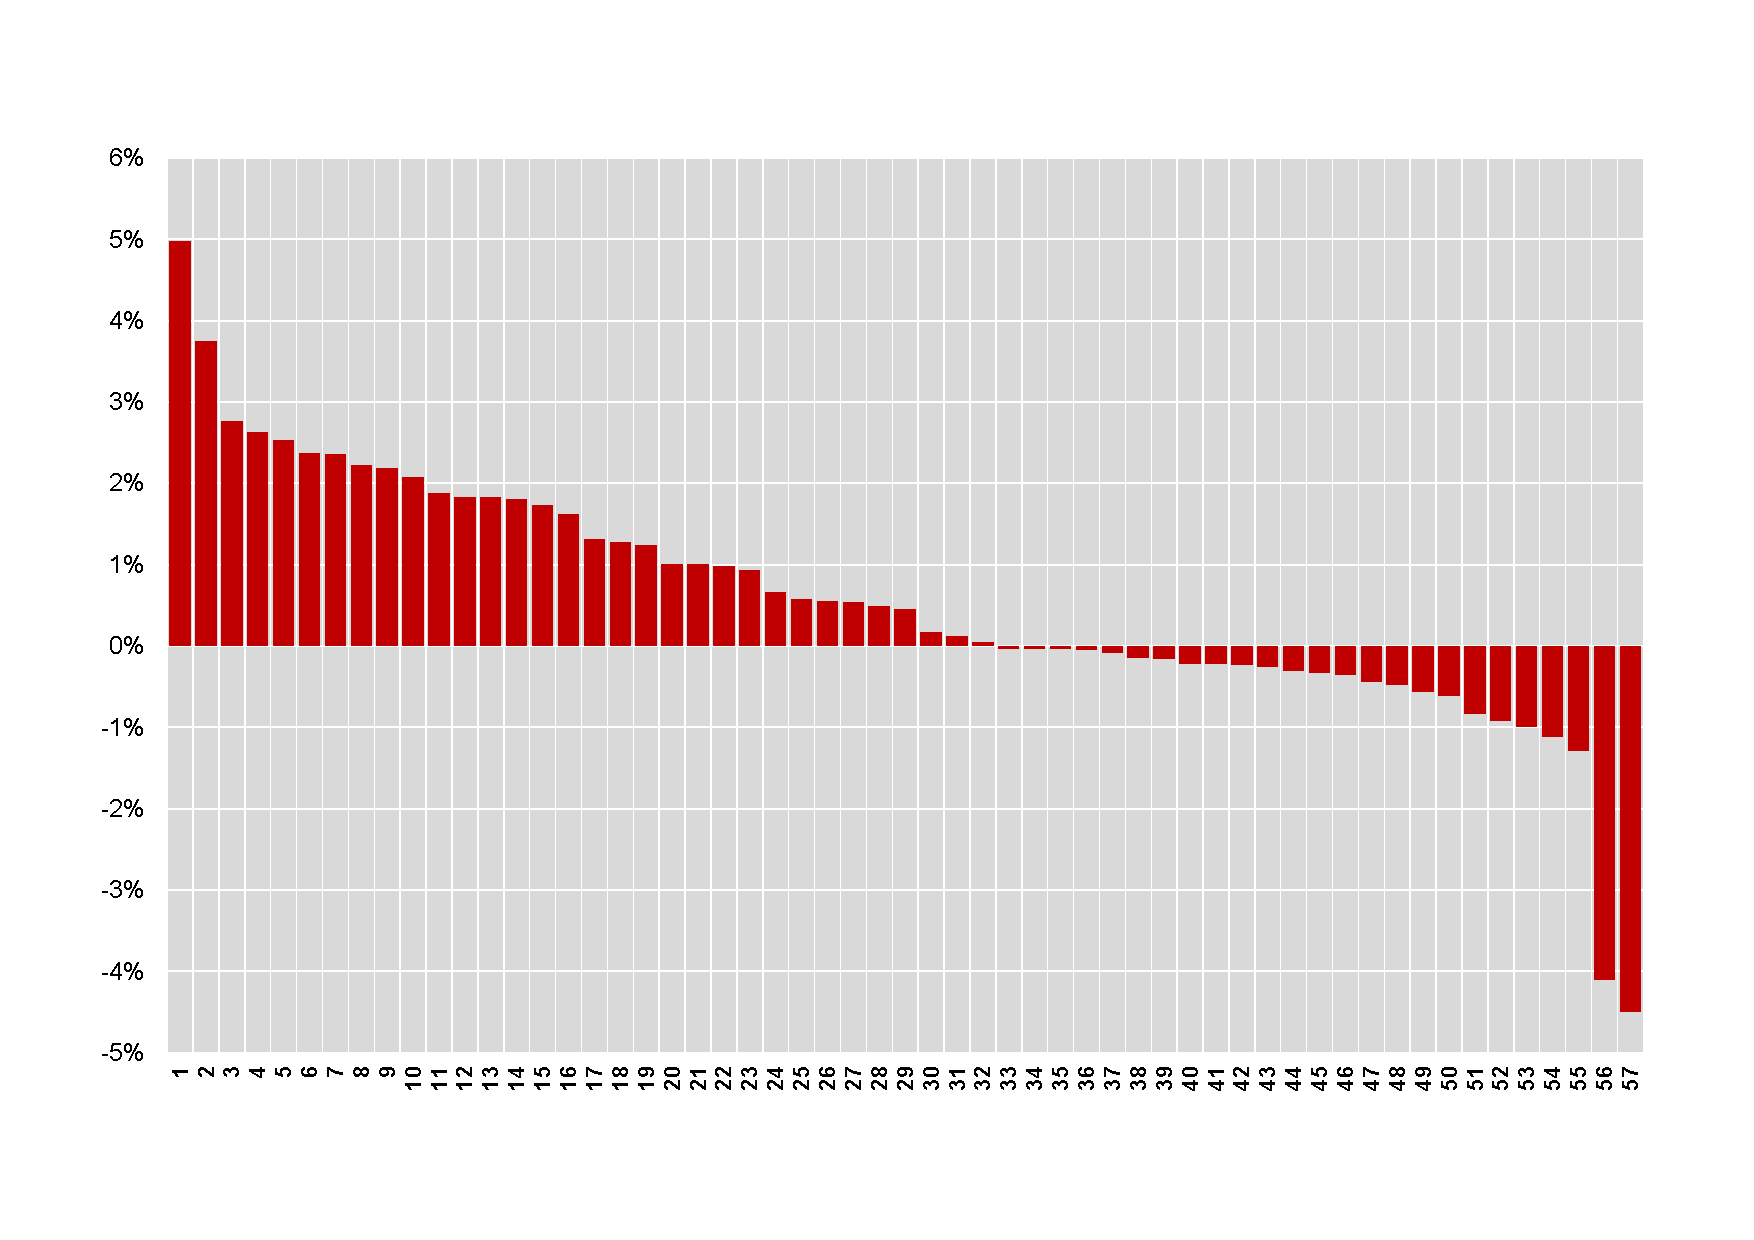
\includegraphics[scale=0.8]{mod_estatico_prod.pdf}
    \caption[Modelo CGE: Produção]{\textbf{Modelo CGE: Produção}. Variação percentual cumulativa da produção real, por setor GTAP, 20 anos após o choque de abertura comercial. \scriptsize{1. Carvão; 2. Pescados; 3. Ferro e aço; 4. Madeira; 5. Papel; 6. Carne in natura; 7. Frutas e vegetais; 8. Arroz processado; 9. Arroz in natura; 10. Outros minérios; 11. Couro; 12. Outros grãos; 13. Trigo; 14. Fibras vegetais; 15. Cana de açúcar; 16. Produtos de metal; 17. Automóveis e peças; 18. Outras colheitas; 19. Equipamentos eletrônicos; 20. Gás; 21. Petróleo; 22. Oleaginosas; 23. Pecuária; 24. Lã; 25. Minerais não-metálicos; 26. Eletricidade; 27. Derivados do petróleo; 28. Outras carnes; 29. Vestuário; 30. Residências; 31. Produtos florestais; 32. Seguros; 33. Outras manufaturas; 34. Transportes aeroviários; 35. Comunicações; 36. Governo; 37. Construção; 38. Intermediação financeira; 39. Serviços comerciais; 40. Químicos; 41. Recreação; 42. Distribuição de gás; 43. Água; 44. Comércio; 45. Laticínios; 46. Outros transportes; 47. Outros maquinários; 48. Açúcar; 49. Óleos vegetais; 50. Outros equip. de transporte; 51. Outros produtos animais; 52. Transportes aquaviários; 53. Metais não ferrosos; 54. Outros alimentos; 55. Leite; 56. Têxteis; 57. Bebidas e tabaco. 
}}
    \label{fig:mod_estatico_prod}
\end{figure}
\end{landscape}
\newpage

\begin{landscape}
\begin{figure}[htbp]
    \centering
    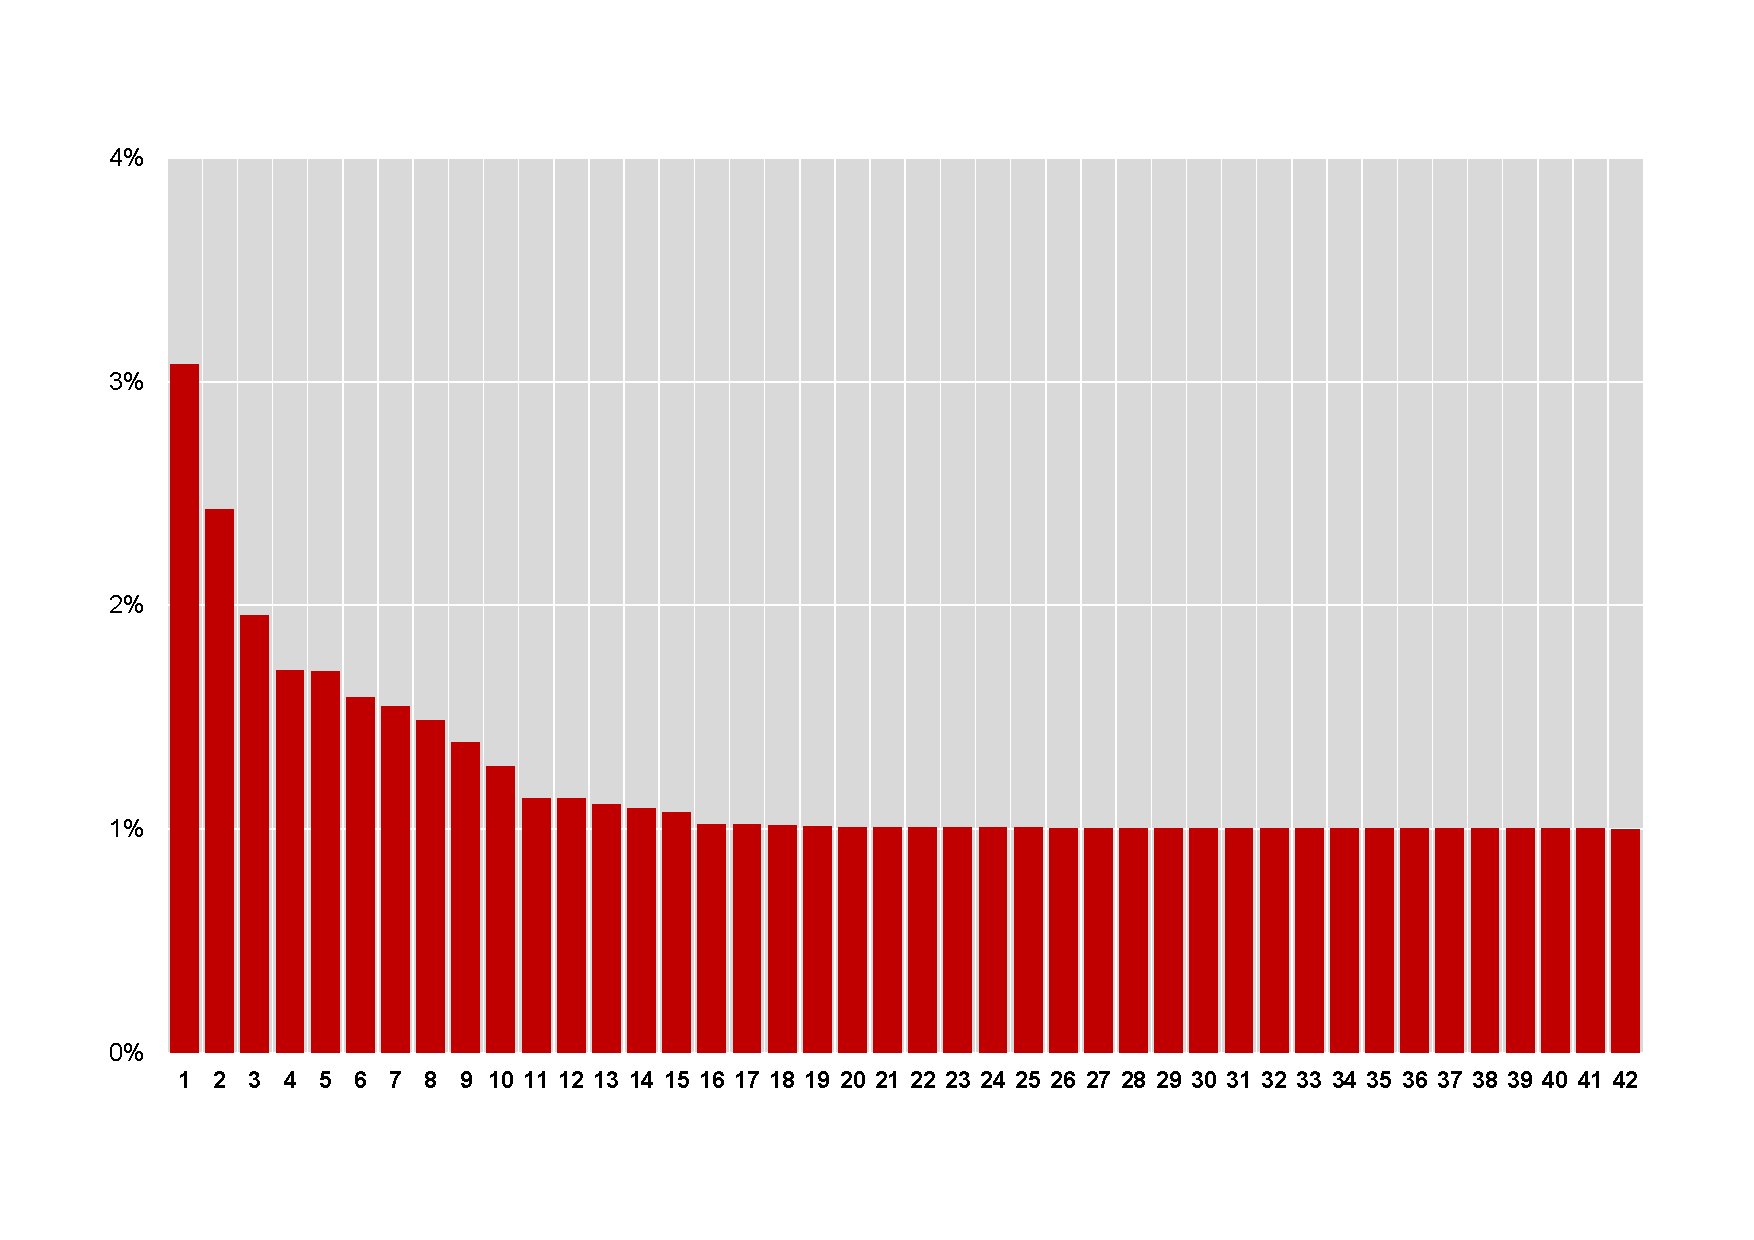
\includegraphics[scale=0.8]{mod_estatico_exp.pdf}
    \caption[Modelo CGE: Exportações]{\textbf{Modelo CGE: Exportações}. Variação percentual cumulativa das exportações reais, por setor GTAP, 20 anos após o choque de abertura comercial. \scriptsize{1. Vestuário; 2. Têxteis; 3. Couro; 4. Madeira; 5. Papel; 6. Equipamentos eletrônicos; 7. Outros maquinários; 8. Produtos de metal; 9. Derivados do petróleo; 10. Outras manufaturas; 11. Químicos; 12. Ferro e aço; 13. Minerais não-metálicos; 14. Metais não ferrosos; 15. Automóveis e peças; 16. Trigo; 17. Outros equip. de transporte; 18. Frutas e vegetais; 19. Outras carnes; 20. Outras colheitas; 21. Outros alimentos; 22. Pecuária; 23. Outros grãos; 24. Leite; 25. Gás; 26. Produtos florestais; 27. Açúcar; 28. Laticínios; 29. Pescados; 30. Arroz processado; 31. Oleaginosas; 32. Petróleo; 33. Bebidas e tabaco; 34. Carvão; 35. Carne in natura; 36. Fibras vegetais; 37. Cana de açúcar; 38. Outros produtos animais; 39. Outros minérios; 40. Óleos vegetais; 41. Lã; 42. Arroz in natura. }}
    \label{fig:mod_estatico_exp}
\end{figure}
\end{landscape}
\newpage

\begin{landscape}
\begin{figure}[htbp]
    \centering
    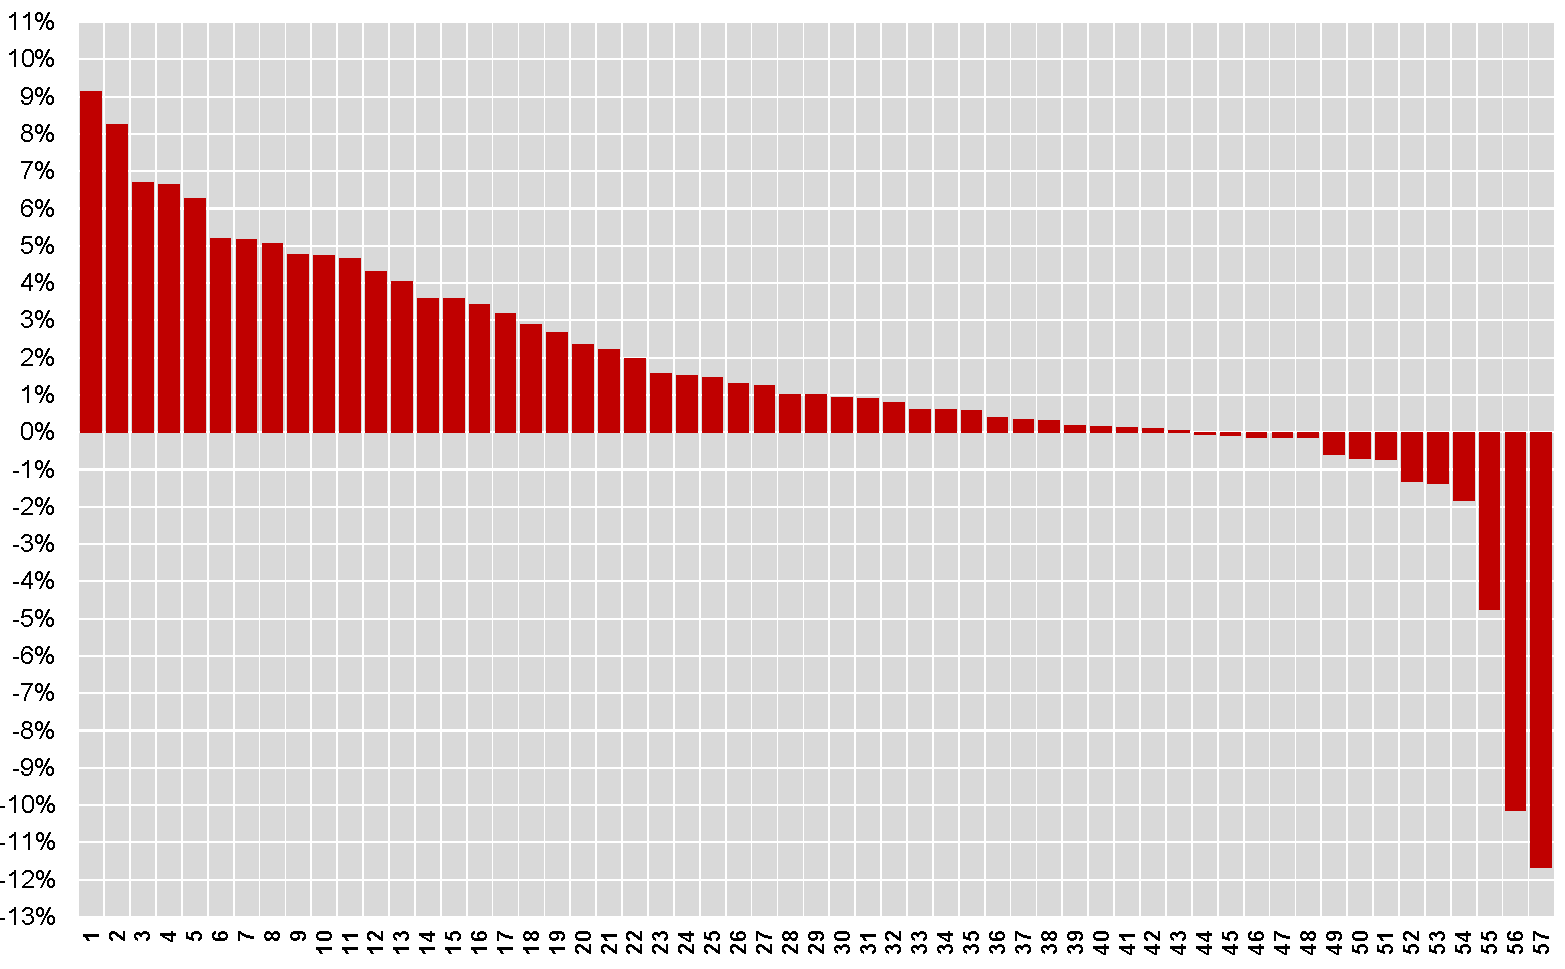
\includegraphics[scale=0.8]{mod_estatico_sal.pdf}
    \caption[Modelo CGE: Salários]{\textbf{Modelo CGE: Salários}. Variação percentual cumulativa dos salários reais, por setor GTAP, 20 anos após o choque de abertura comercial. \scriptsize{1. Carvão; 2. Pescados; 3. Papel; 4. Frutas e vegetais; 5. Arroz in natura; 6. Trigo; 7. Fibras vegetais; 8. Ferro e aço; 9. Outros minérios; 10. Carne in natura; 11. Arroz processado; 12. Outras colheitas; 13. Madeira; 14. Outros grãos; 15. Oleaginosas; 16. Pecuária; 17. Cana de açúcar; 18. Outras carnes; 19. Eletricidade; 20. Lã; 21. Produtos florestais; 22. Automóveis e peças; 23. Couro; 24. Minerais não-metálicos; 25. Outras manufaturas; 26. Derivados do petróleo; 27. Açúcar; 28. Gás; 29. Petróleo; 30. Comércio; 31. Outros transportes; 32. Laticínios; 33. Transportes aquaviários; 34. Químicos; 35. Seguros; 36. Transportes aeroviários; 37. Distribuição de gás; 38. Comunicações; 39. Construção; 40. Residências; 41. Óleos vegetais; 42. Outros produtos animais; 43. Intermediação financeira; 44. Água; 45. Serviços comerciais; 46. Recreação; 47. Governo; 48. Leite; 49. Outros alimentos; 50. Outros equip. de transporte; 51. Produtos de metal; 52. Outros maquinários; 53. Equipamentos eletrônicos; 54. Metais não ferrosos; 55. Vestuário; 56. Bebidas e tabaco; 57. Têxteis.}}
    \label{fig:mod_estatico_sal}
\end{figure}
\end{landscape}
\newpage

\subsection{Resultados heterogêneos regionais sobre o mercado de trabalho}

Apesar do baixo impacto agregado esperado da liberalização comercial no mercado de trabalho do país, podem ocorrer efeitos negativos localizados. Isso porque: (1) os custos do ajuste ocorrem setores da economia que são espacialmente concentrados; e (2) os ajustes no mercado de trabalho tem se mostrado mais lentos do que se tinha como consenso da literatura sobre o efeito de choques de comércio. 

Os elementos discutidos acima enfatizam a necessidade de estimar a distribuição espacial dos efeitos da liberalização sobre o mercado de trabalho.  Para tanto, após computados os resultados esperados da abertura comercial no nível nacional, foram utilizados dados da Relação Anual de Informações Sociais (RAIS) para estimar os efeitos esperados da abertura sobre o emprego em distintas regiões do País. Combinando o fato de os 57 setores incluídos na simulação apresentada anteriormente serem geograficamente concentrados com a relação histórica entre as flutuações de emprego em cada região-setor e as variações nacionais de emprego em cada setor, é possível estimar qual o efeito esperado sobre o emprego total de cada região após a liberalização comercial.  

O propósito desse exercício é identificar prospectivamente onde estão os trabalhadores que serão negativamente afetados pela transição a uma estrutura comercial moderna, para que o poder público possa traçar políticas de requalificação e reinserção destes trabalhadores no mercado de trabalho. Como visto, há evidências empíricas de que, na ausência de uma política de proteção destes trabalhadores, o processo de ajuste pode ser muito lento, já que não há plena mobilidade geográfica no mercado de trabalho. A lógica subjacente, portanto, é que possam ser alcançados os ganhos agregados com o comércio sem que trabalhadores específicos sejam desproporcionalmente penalizados pelos custos da transição.

Em cerca de dois terços das 558 microrregiões brasileiras, estima-se que o efeito de longo prazo da liberalização sobre o emprego formal é positivo (ver Figura \ref{fig:mapa_micro}). Este efeito, contudo, tende a ser pequeno. Em 85\% das microrregiões o efeito se concentra no intervalo de -0,25\% a +0,25\% de variação no emprego formal. Mesmo os casos mais extremos variam entre -2\% e +2\% da força de trabalho.

O exercício permite identificar que em algumas regiões o efeito se distancia da média. O Centro-Oeste, de um modo geral, se coloca um pouco acima da média nacional, assim como o Sul do Piauí e do Maranhão e algumas microrregiões do Pará, Amazonas, Roraima e Amapá, com ganhos de emprego formal que chegam a 2\%. Nas outras regiões, o efeito esperado é \textit{grosso modo} nulo, com exceção do Vale do Itajaí (SC), Sul da Bahia e um aglomerado de microrregiões do Noroeste Cearense, nas quais poderá ocorrer perda de emprego formal em setores atualmente instalados.

As microrregiões que se concentram nos extremos positivo e negativo quanto à variação esperada sobre o emprego tendem a ser menores em termos populacionais. Cidades maiores tendem a ter resultado muito próximo a zero (ver Figura \ref{fig:percentil}). Esse resultado é intuitivo, uma vez que metrópoles tendem a ter economias mais diversificadas e, frente ao choque imposto pela abertura comercial, os trabalhadores conseguem simplesmente migrar de setores, dentro da mesma microrregião, sendo o resultado líquido nulo (ver Figura \ref{fig:mapa_micro}).

\newpage
\begin{figure}[htbp!]
    \centering
    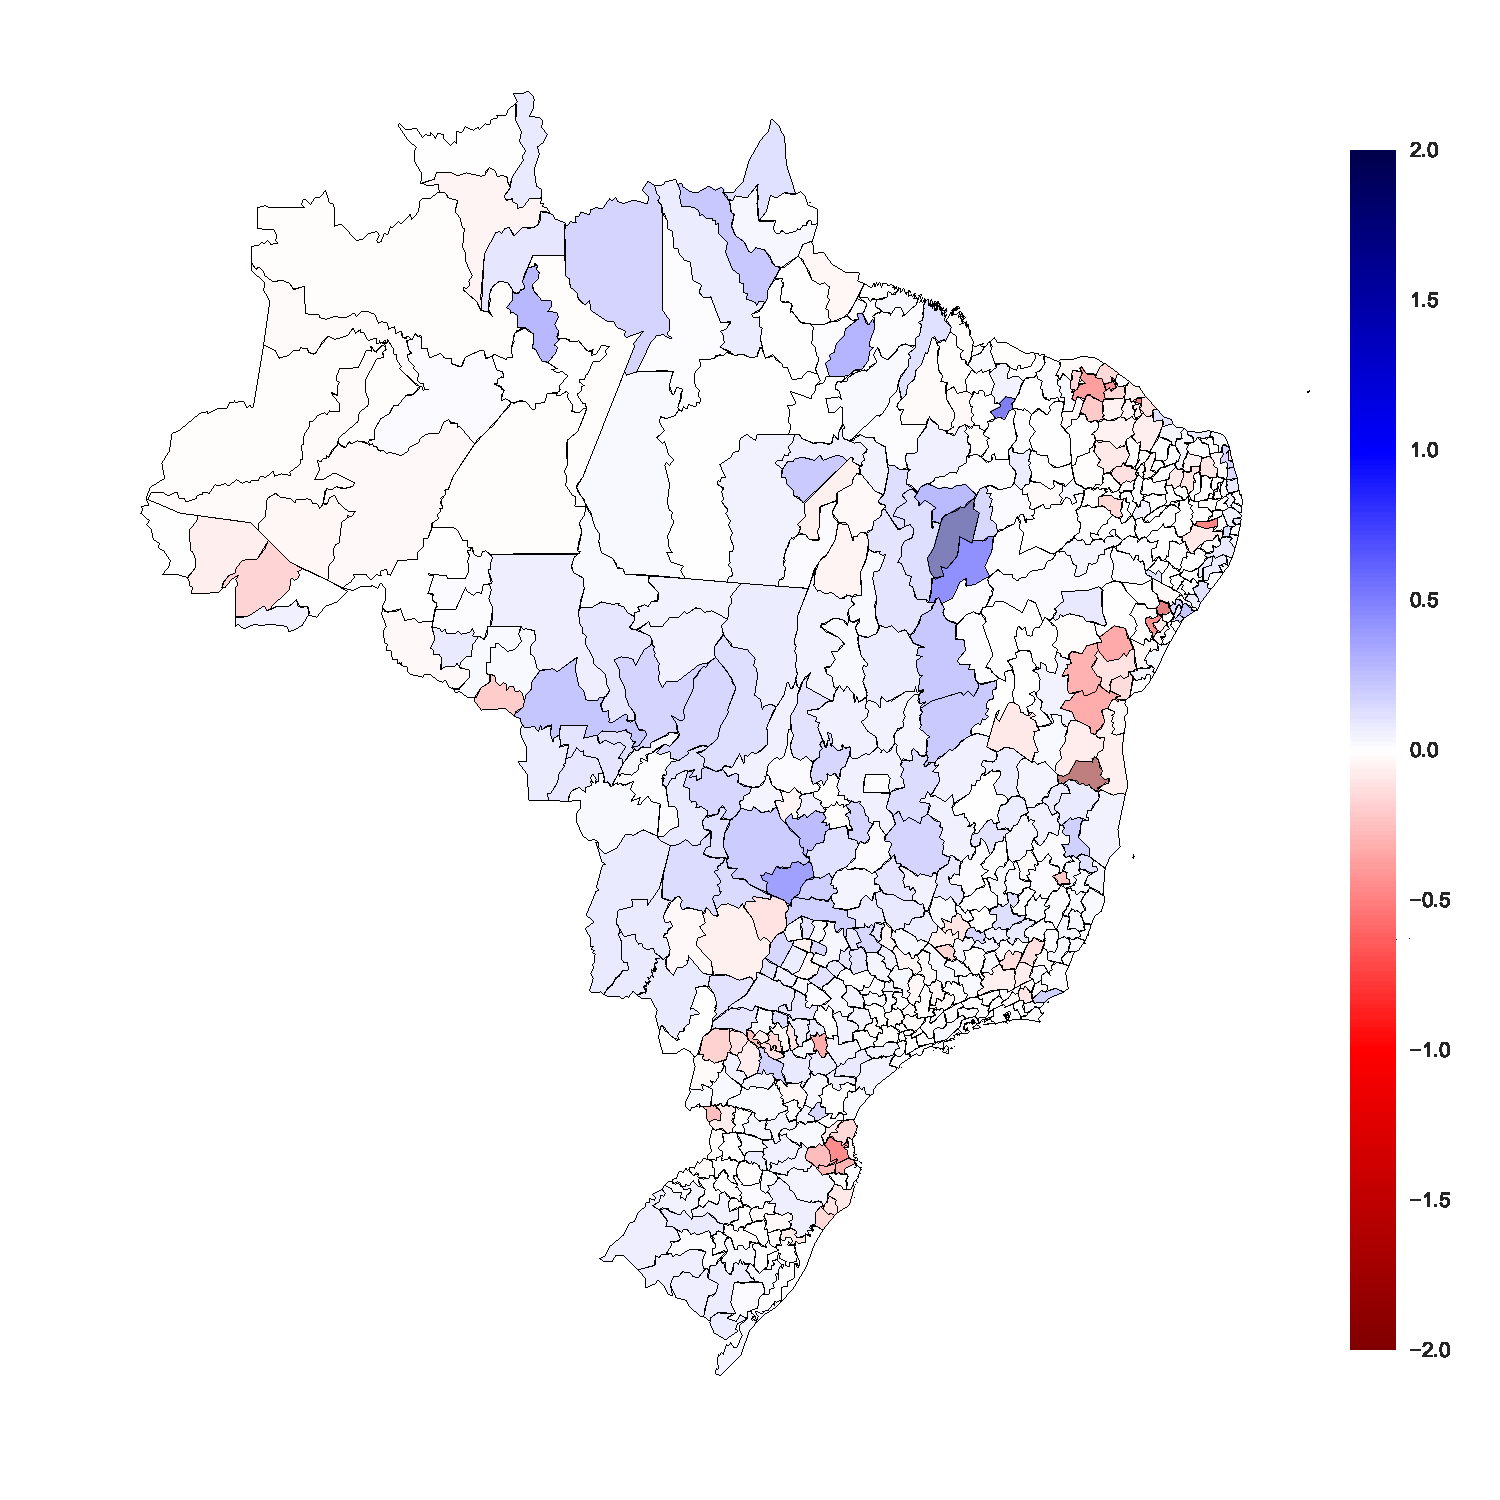
\includegraphics[scale=0.68]{mapa_micro.pdf}
    \caption[Resultados locais: distribuição geográfica dos efeitos sobre a população ocupada]{\textbf{Resultados locais: distribuição geográfica dos efeitos sobre a população ocupada}. Variação percentual cumulativa líquida na população ocupada, por microrregião, 20 anos após o choque de abertura comercial. }
    \label{fig:mapa_micro}
\end{figure}
\newpage

\begin{landscape}
\begin{figure}[htbp]
    \centering
    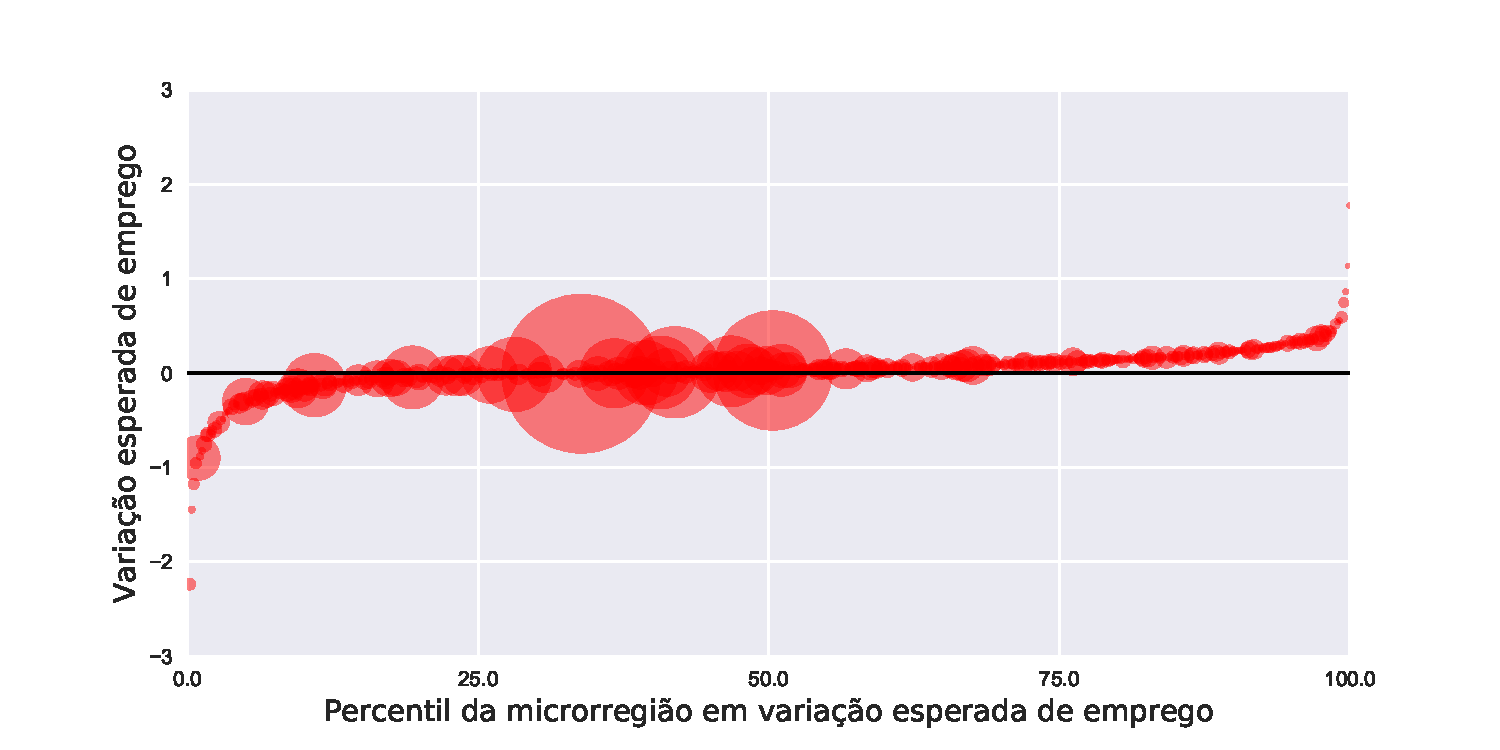
\includegraphics[scale=1]{laborforce.pdf}
    \caption[Resultados locais: população ocupada, percentil e tamanho da força de trabalho]{\textbf{Resultados locais: população ocupada, percentil e tamanho da força de trabalho}. xxxx.}
    \label{fig:percentil}
\end{figure}
\end{landscape}
\newpage

Esses resultados divergentes se explicam, em grande parte, pela concentração regional dos distintos setores da economia brasileira e seus distintos níveis tarifários. Microrregiões têm níveis distintos de proteção comercial – aquelas que concentram sua força de trabalho e produção regional em setores com tarifas mais altas têm um nível de proteção mais alto. Essas microrregiões são aquelas que tenderão a ser mais afetadas pela liberalização comercial.

Utilizando a metodologia descrita em \textcite{dixkovak} e \textcite{kovak}, é possível calcular o nível de proteção tarifária para cada microrregião, ao ponderar-se as tarifas nacionalmente aplicadas à importação de diversos bens e serviços com a composição setorial da força de trabalho regional. O choque choque comercial que se segue à eliminação dos níveis tarifários vigentes define-se da seguinte maneira:

\begin{eqnarray}
    \hat{w}_{m,s,g} &=& \sum_{m,s}^{M_s,S} \beta_{m,s} \hat{P}_g \\
    \beta_{m,s,g} &=& \frac{ \lambda_{m,s,g} \frac{1}{\varphi_{m,s}} }{ \sum_{m,s}^{M_s,S} \lambda_{m,s,g}\frac{1}{\varphi_{m,s} }}
\end{eqnarray}

em que, para cada setor GTAP \(g\) em cada microrregião dos distintos estados \(r,g\): \(\lambda_{m,s,g}\) é a proporção inicial do trabalho alocado no setor  \(g\) na microrregião \(m,s\), que é heterogênea entre micorregiões; \(\varphi_{m,s}\) é a remuneração dos fatores excetuando trabalho no setor \(g\), que é heterogênea entre setores diferentes; e \(\hat{P}_g\) é a variação percentual nos preços do setor \(g\) causada pela mudança tarifária.

O cálculo de uma tarifa regional heterogêna, que é eliminada no processo de liberalização comercial, portanto, pode ser calculado utilizando-se a variação tarifária esperada para  distintos setores da economia nacional:

\begin{eqnarray}
    \label{eq:reg_tar}
    \tau_{m,s} &=& \sum_{m,s}^{M_s,S} \beta_{m,s,g} \Delta \ln(1+\tau_\tau_{m,s,g}) \nonumber \\
    \tau_{m,s} &=& \sum_{m,s}^{M_s,S} \beta_{m,s,g} [\ln (1 + \tau_{m,s,g}^{t+k}) - \ln (1 + \tau_{m,s,g}^{t})] \\
    \tau_{m,s,g}^{t+k} &\equiv& \tau_{g}^{t+k} \qquad \forall \qquad m,s,t \nonumber 
\end{eqnarray}


onde \(\tau_{m,s,g}^{t}\) indica a tarifa inicial e \(\tau_{m,s,g}^{t+k}\) a tarifa no ano \(t+k\) para o setor $g$ \textemdash sendo as tarifas iniciais e finais homogêneas para todas as microrregiões, uma vez que elas são determinadas no nível nacional. A substituição de \emph{variação de preço} por \emph{variação na tarifa} pode ser pensado como ``a reduced-form analysis in which tariff changes act as exogenous instruments for price changes faced by producers.'' \parencite{kovak}.

Para cada microrregião, deriva-se uma tarifa regional ($\tau_{m,s}$) para o ano base da simulação. Os parâmetros $\lambda_{m,s,g}$ são consolidados de microdados do censo laboral anual (RAIS), que descreve o número de empregados para distintos setores da economia, tomando-se como base a matriz de correspondência entre os códigos da RAIS e do GTAP (ver Apêndice \ref{appendix:CNAEGTAP} para detalhes). Seguindo \textcite{dixkovak}, que argumentam e apresentam evidências de que os preços dos bens não-comerciáveis seguem os dos comerciáveis, os setores não-comercializáveis são excluídos da análise,   de tal modo que $\sum_{m,s}^{M_s,S} \beta_{m,s,g} = 1$ para o conjunto de setores comercializáveis.

Com isso, percebe-se que a distribuição geográfica do protecionismo tarifário brasileiro tem grande variação (ver Figura \ref{fig:mapa_micro_tarifa}). Cerca de 50\% das microrregiões têm proteção tarifária menor que 8,7\%, 80\% têm proteção tarifária menor que 12\% e 90\% têm proteção tarifária menor que 15\%, restando algumas poucas microrregiões específicas com níveis de proteção muito mais alto, ultrapassando o equivalente a uma tarifa ad valorem de 20\% (ver Figura \ref{fig:rtr_hist}).

\begin{figure}[ht!]
    \centering
    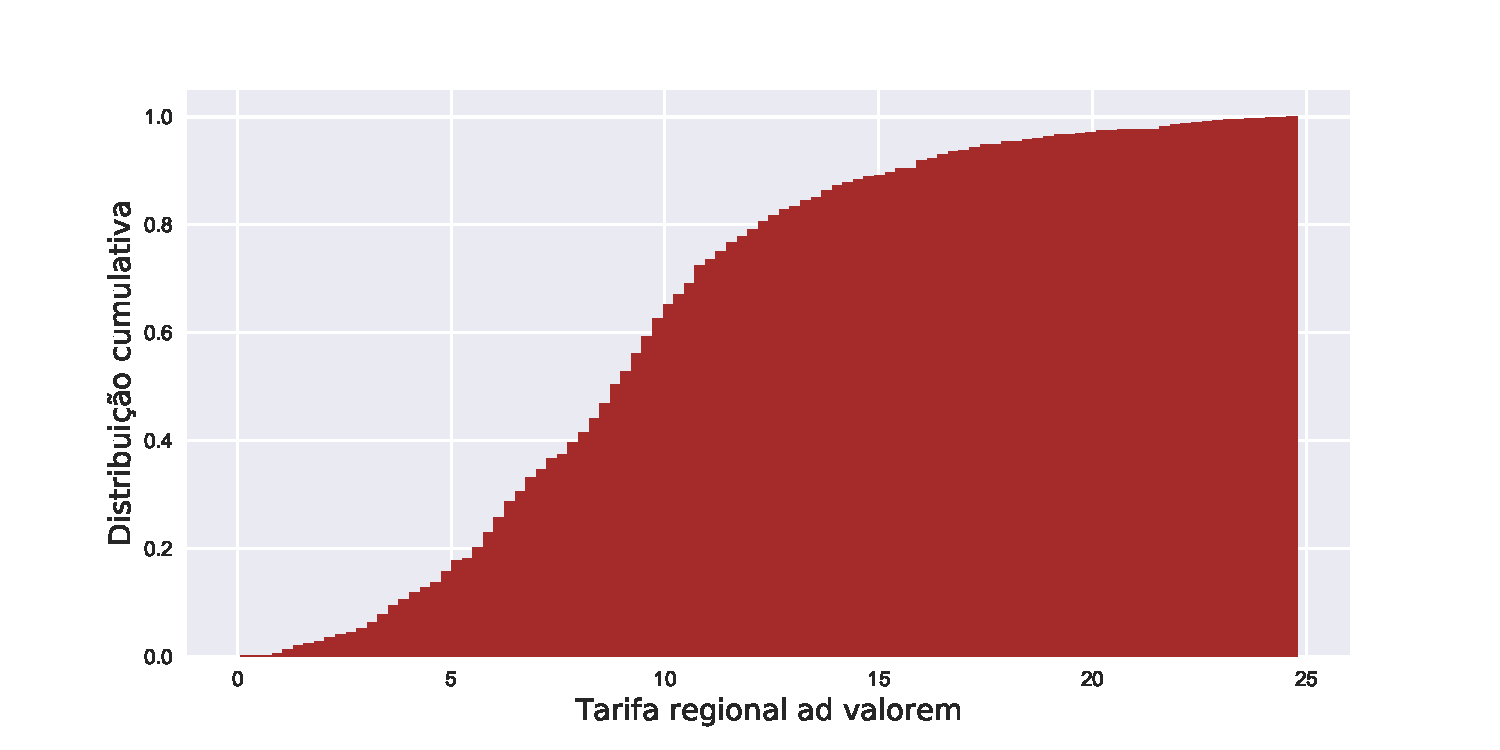
\includegraphics[scale=0.55]{rtr_hist.pdf}
    \caption[Tarifas regionais: distribuição cumulativa das microrregiões]{\textbf{Tarifas regionais: distribuição cumulativa das microrregiões}. Distribuição cumulativa do número de microrregiões para cada nível de proteção comercial.}
    \label{fig:rtr_hist}
\end{figure}

A análise se altera um pouco na cauda esquerda da distribuição quando é feita a ponderação pela força de trabalho de cada uma das microrregiões. Cerca de 50\% da força de trabalho reside em microrregiões com proteção tarifária menor que 10,69\%. Na cauda direita, contudo, há pouca modificação: 80\% da força de trabalho tem proteção tarifária menor que 12\% e 90\% têm proteção tarifária menor que 15\% (ver Figura \ref{fig:rtr_hist_w}).

\newpage

\begin{figure}[htbp!]
    \centering
    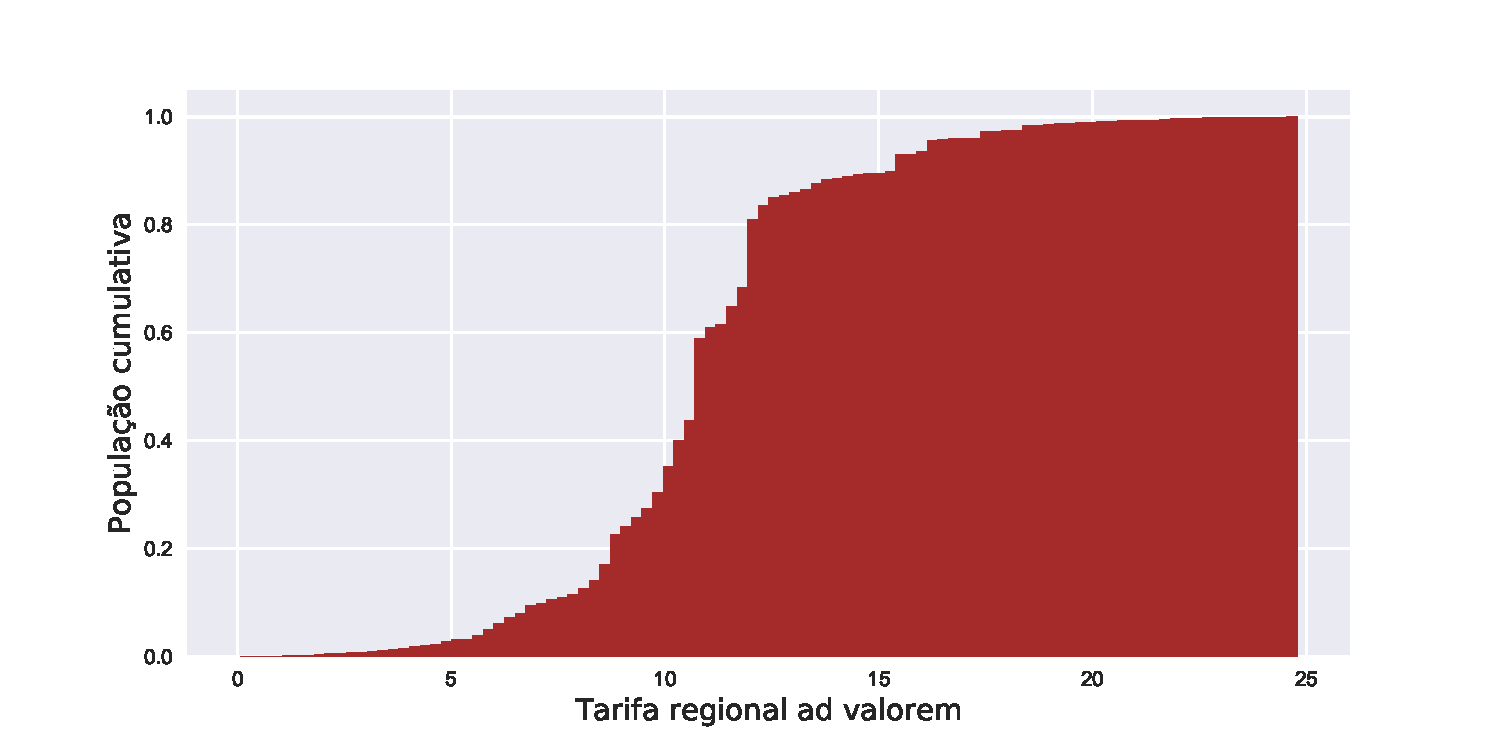
\includegraphics[scale=0.55]{rtr_hist_w.pdf}
    \caption[Tarifas regionais: distribuição cumulativa da força de trabalho]{\textbf{Tarifas regionais: distribuição cumulativa da força de trabalho}. Distribuição cumulativa do número de microrregiões para cada nível de proteção comercial, ponderada pela força de trabalho de cada microrregião.}
    \label{fig:rtr_hist_w}
\end{figure}

Os efeitos estimados na equação (\ref{eq:micro_agg}), que combinam os choques agregados derivados do modelo de EGC com as elasticidades estimadas no modelo empírico (\ref{equation:painel}), têm correlação negativa com as tarifas regionais calculadas na equação (\ref{eq:reg_tar}). A correlação é fortemente significante ($|t-valor| > 9$) e persiste mesmo quando controlada pelo tamanho da força de trabalho do município ou sua renda familiar per capita. O sinal da correlação é conforme o esperado, uma vez que é razoável que regiões que hoje têm maior proteção tarifária observem uma contração maior na força de trabalho no longo prazo.

Esses resultados vão no mesmo sentido das conclusões de \textcite{dixkovak}, que demonstraram que as regiões que sofreram um maior choque comercial durante o processo de liberalização dos anos 1990 tiveram uma perda relativa de emprego formal em face às outras regiões do país. Esse fato estilizado indica que a presente análise prospectiva conseguiu incorporar de forma eficiente as conclusões empíricas da literatura em relação à heterogeneidade regional dos choques de preços relativos que se seguem a um processo de liberalização comercial.

\newpage

\begin{figure}[htbp!]
    \centering
    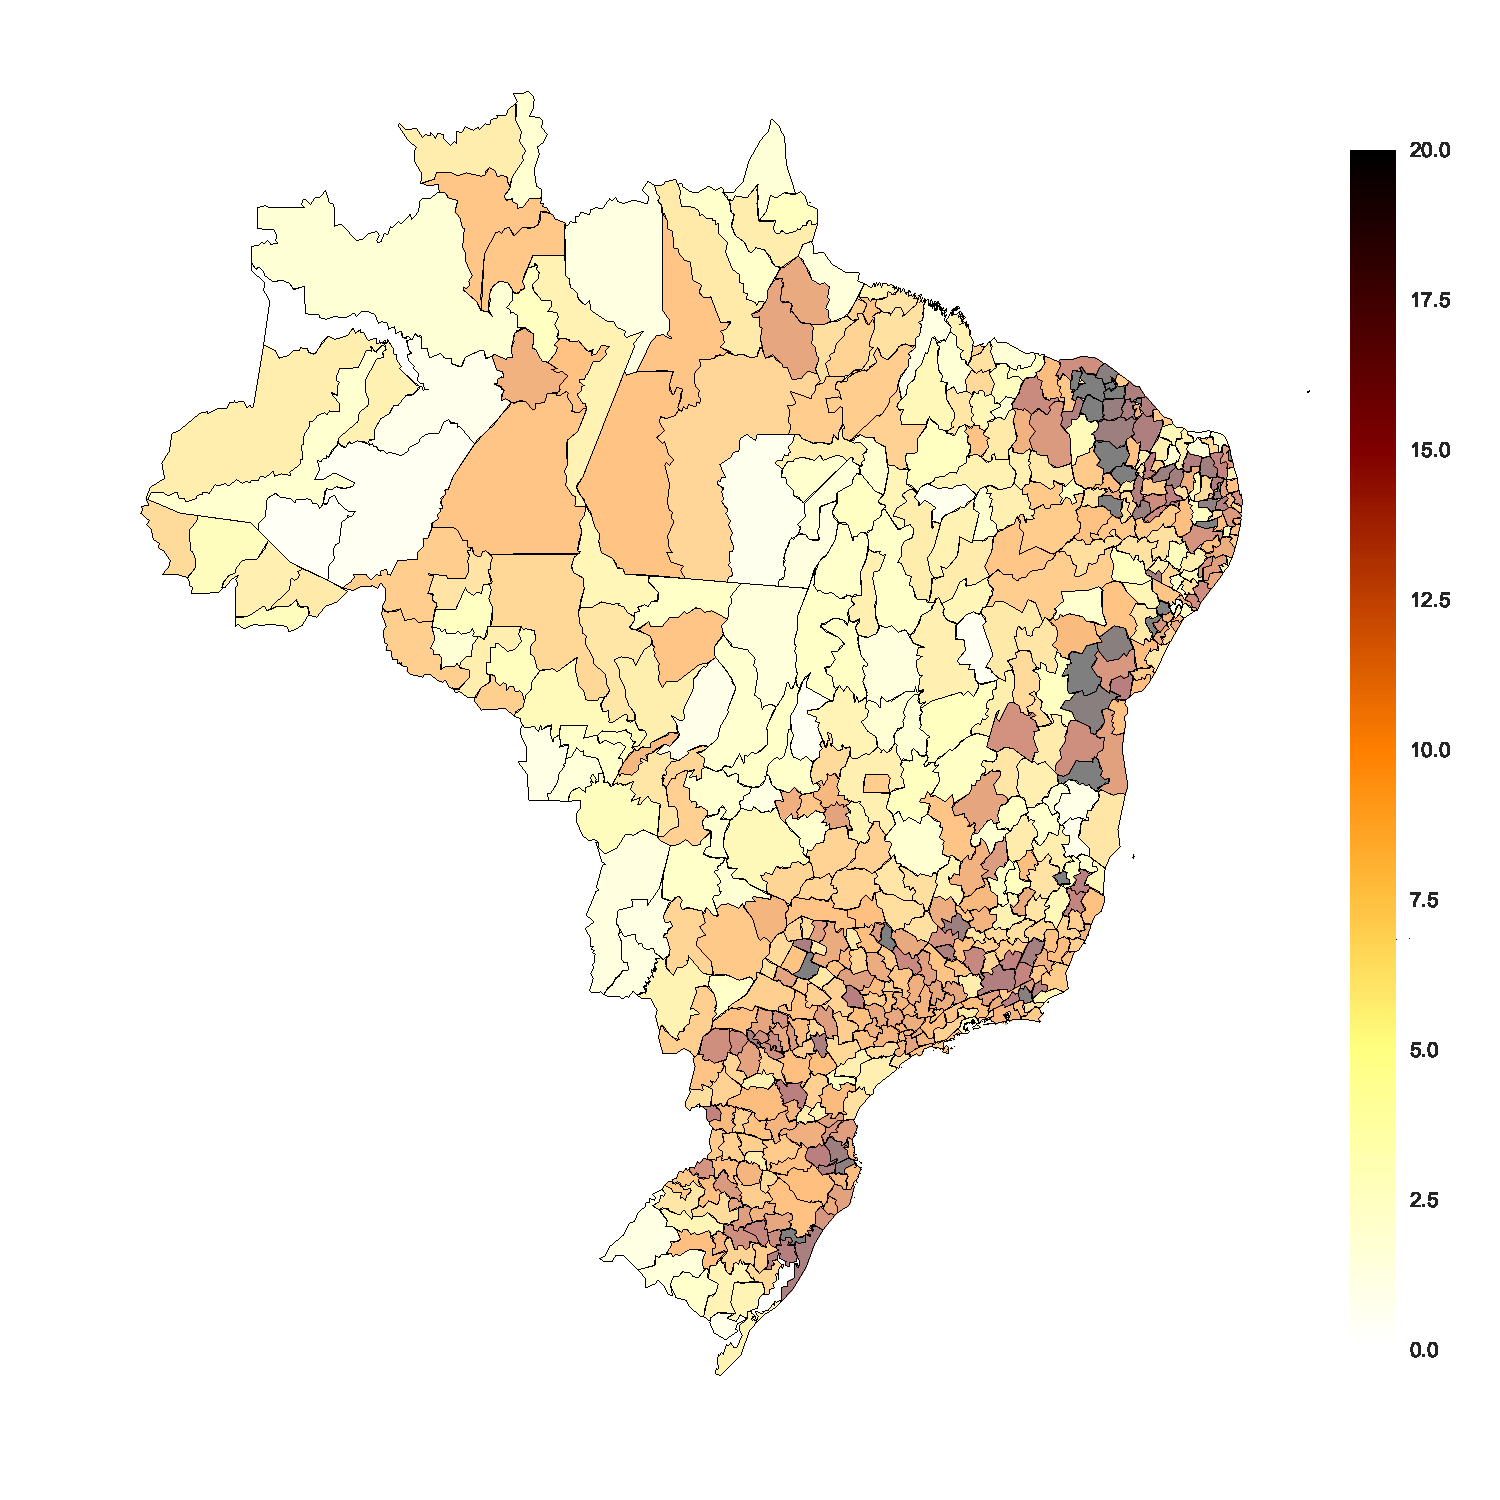
\includegraphics[scale=0.68]{mapa_micro_tarifa.pdf}
    \caption[Resultados locais: tarifas regionais]{\textbf{Resultados locais: tarifas regionais}. Tarifa \textit{ad valorem} efetiva para cada microrregião brasileira, ponderada pela alocação setorial da força de trabalho em cada microrregião. }
    \label{fig:mapa_micro_tarifa}
\end{figure}

\newpage

\begin{landscape}
\begin{figure}[htbp]
    \centering
    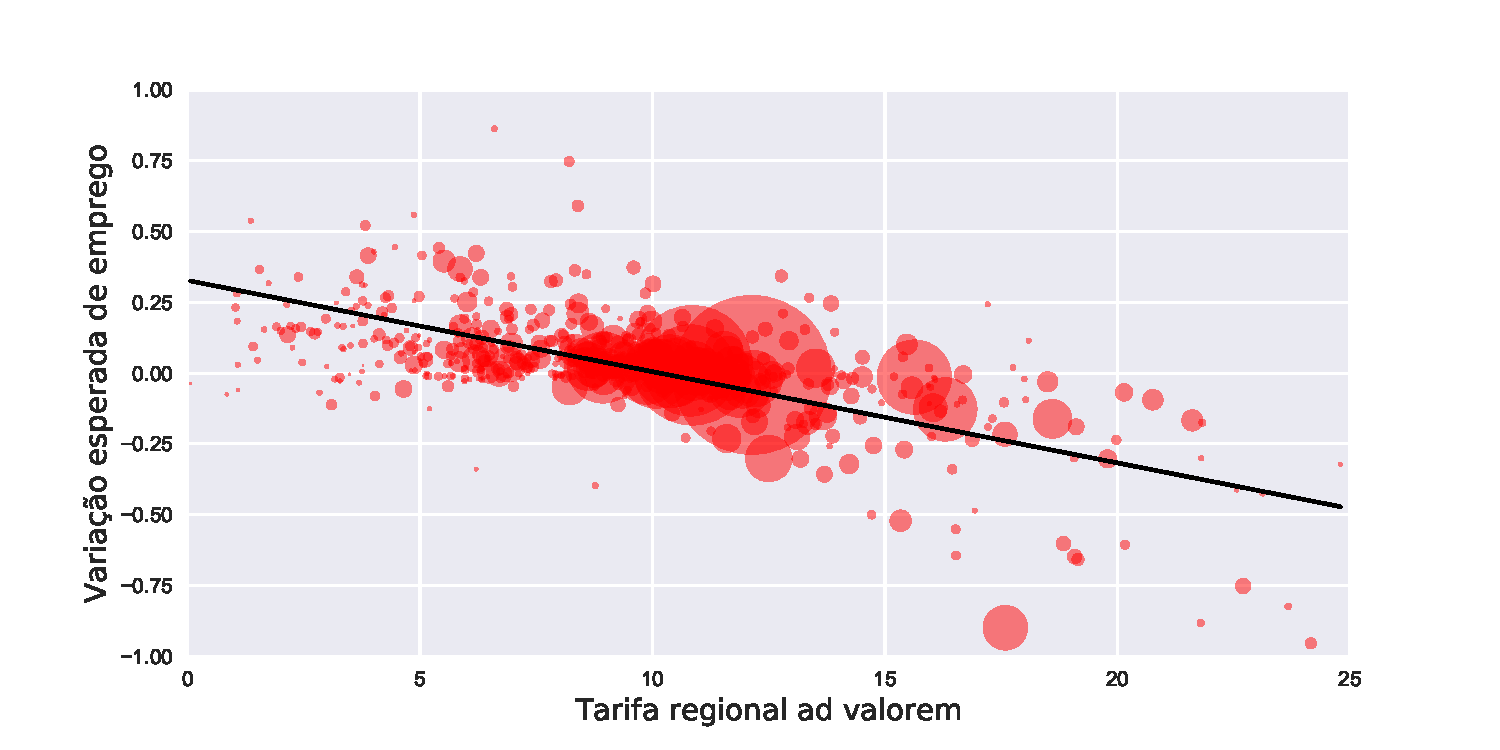
\includegraphics[scale=1]{rtr_effects.pdf}
    \caption[Resultados locais: população ocupada, percentil e tamanho da força de trabalho]{\textbf{Resultados locais: população ocupada, percentil e tamanho da força de trabalho}. xxxx.}
    \label{fig:rtr_effects}
\end{figure}
\end{landscape}

\section{Conclusões e implicações de política pública} 

Partindo de um Modelo de Equilíbrio Geral Computável com fricções laborais e heterogeneidade em produtividade, este trabalho desenvolve uma estratégia metodológica para de estimação de efeitos regionais heterogêneos de uma liberalização comercial sobre o mercado de trabalho numa análise prospectiva, mesmo na ausência de matrizes regionais de insumo-produto. Nesse sentido, ele se arvora sobre inovações realizadas sobre duas diferentes linhas de pesquisa em economia internacional, quais sejam: a incorporação de fricções e heterogeneidade nos modelos de análise prospectiva e de efeitos laborais regionalmente heterogêneos de choques comerciais nos modelos empíricos retrospectivos.

Após a estimação de 1.539 elasticidades heterogêneas específicas para cada díade estado-setor, calculou-se o efeito esperado para cada setor em cada microrregião ao combinar-se o tamanho do choque nacional para cada setor com as elasticidades específicas. Ao agregar-se os efeitos esperados de cada um dos 57 setores para cada uma das microrregiões, foi possível estimar o efeito líquido esperado sobre o emprego formal para cada microrregião.

Os resultados indicam relativa heterogeneidade nos efeitos regionais sobre o mercado de trabalho. Em cerca de dois terços das 558 microrregiões brasileiras, estima-se que o efeito de longo prazo da liberalização sobre o emprego formal é positivo. Este efeito, contudo, tende a ser pequeno. 

A heterogeneidade dos efeitos regionais estimada, que se explica em grande medida pela concentração espacial dos distintos setores da economia brasileira, vai no mesmo sentido das conclusões de \textcite{dixkovak}: regiões que atualmente têm uma proteção comercial regional mais elevada tenderão a observar efeitos relativamente maiores sobre seu mercado de trabalho.

O método aqui desenvolvido, que pode ser expandido para outros países desde que dados setoriais sobre os mercados de trabalho regionais estejam disponíveis, tem importantes implicações de política pública. Ao incorporar prospectivamente a heterogeneidade regional de uma abertura comercial, os tomadores de decisão podem tentar antecipar tais efeitos díspares e desenhar políticas ativas para o mercado de trabalho que amenizem o efeito da liberalização comercial nas regiões mais afetadas e facilitem a migração intersetorial e interregional de trabalhadores. Assim, seria possível que fossem alcançados os ganhos agregados com o comércio sem que trabalhadores específicos sejam desproporcionalmente penalizados pelos custos da transição para uma economia mais aberta.

\printbibliography

\newpage

\appendix
\numberwithin{equation}{section}
\section{Apêndice: Dados e Fontes}

\subsection{Dados utilizados para estimação dos efeitos sobre o mercado de trabalho regional}

Os dados de produção e comércio utilizados na presente análise foram extraídos da base do Global Trade Analysis Project (GTAP), versão 9 (ano-base 2011). Cada simulação envolveu 27 regiões econômicas: África do Sul, Arábia Saudita, Argentina, Bolívia, Brasil, Canadá, Chile, China, Colômbia, Coréia do Sul, Egito, Estados Unidos, Índia, Indonésia, Japão, Malásia, México, Nigéria, Paraguai, Peru, Rússia, Suíça, Turquia, Uruguai, Vietnã, União Europeia, e o restante do mundo agrupado como uma única região. Com isso, dessas 27 regiões econômicas, de forma desagregada em 57 setores (conforme a desagregação máxima da GTAP Sectoral Classification, Revision 2), foram extraídos os dados referentes a: produção doméstica, matriz de insumo-produto, fluxos comerciais bilaterais e tarifas bilaterais.

Por sua vez, os dados referentes ao mercado de trabalho foram extraídos da Relação Anual de Informações Sociais (RAIS), do Ministério do Trabalho e Previdência Social. A RAIS é um censo anual do mercado laboral brasileiro, existente desde 1976, que tem como objetivo organizar informações individualizadas sobre toda a população de trabalhadores empregados no mercado formal.

Tal censo laboral se utiliza de formulários entregues pelos empregadores com dados individualizados de cada vínculo de trabalho formal em sua empresa. Como os empregadores estão sujeitos a uma multa no caso de não entregarem os formulários no prazo ou caso entreguem com informações falsas \footnote{Lei nº 7.998, de 1990}, eles têm fortes incentivos para responder ao censo de forma adequada \textemdash e as informações da RAIS podem ser consideradas de alta qualidade.

Em sua versão pública\footnote{Disponível em \url{ftp://ftp.mtps.gov.br/pdet/microdados/RAIS/2015/}} estão disponíveis, entre outros, dados anonimizados de cada trabalhador referentes à atividade econômica da empresa empregadora, salário, idade do trabalhador, entre outros. Utilizamos somente o número de empregados por setor econômico do empregador, incluindo somente os vínculos ativos.\footnote{Cada trabalhador pode ter mais de um vínculo empregatício. Por exemplo, um professor pode lecionar em mais de uma instituição de ensino. Isso pode levar a erros de superestimação de trabalhadores. Em versão futura pretendemos utilizar a versão confidencial da RAIS, que dispõe de um identificador único por trabalhador.}

Para compatibilizar os setores GTAP aos dados da RAIS, construiu-se uma matriz de transição que faz uma correspondência entre os códigos do Cadastro Nacional de Atividades Econômicas (CNAE), disponíveis na RAIS, e os setores GTAP. Com base nas agregações locais e nacionais resultantes dessa matriz, fizemos a calibragem do Modelo de Equilíbrio Geral Computável e as estimações de elasticidade locais.

De modo a conseguir estimar as elasticidades descritas na equação (\ref{equation:painel}) e realizar a calibração do modelo de Equilíbrio Geral Computável, nós construímos séries temporais, extraídas das RAIS entre 2002 e 2015, para cada díade setor-microrregião. Posteriormente, nós criamos agregados nacionais e estaduais, ao somar a força de trabalho setorial de cada um dos estados:

\begin{equation}
    e_{g,t} = \sum_{s=1}^{27} e_{s,g,t} =  \sum_{s=1}^{27} \sum_{m=1}^{M_s} e_{m,s,g,t}
    \label{eq:agg}
\end{equation}

em que $e_{m,s,g,t}$ é o emprego na microrregião $m = [1, \hdots, M_s]$ do estado $s = [1, \hdots, 27]'$, no setor $g = [1, \hdots, 57]'$ e no ano $t = [2002, \hdots, 2015]'$. Com base nessas agregações estaduais e nacionais foram computadas as elasticidades descritas em (\ref{equation:painel}) e os efeitos em cada microrregião descritos em (\ref{eq:micro_agg}).

Para a calibragem do modelo de equlíbrio geral computável, após segregar os trabalhadores por setor GTAP, as migrações intersetoriais foram estimadas por meio da média ponderada de transição dos trabalhadores, considerando os respectivos setores em que eles estavam empregados (ou não) no dia 31 de dezembro de cada ano. Finalmente, para a distribuição de trabalhadores ao longo dos setores foram considerados os dados referentes a dezembro de 2011 (ano-base dos dados de produção e comércio). Já para a estimação das elasticidades, calculamos agregados setoriais para o país e para cada estado, para cada período. Após a construção dessa base de dados foi possível a estimações de elasticidades descrita na seção anterior.

\subsection{Dados utilizados para cálculo da tarifa regional}

Para o cálculo das tarifas regionais descrito na equação (\ref{eq:reg_tar}), foram necessários três componentes distintos: as variações tarifárias, a composição da força de trabalho para cada microrregião e a remuneração dos fatores em cada setor.

Para calibrar os choques regionais, utilizamos como tarifas iniciais por GTAP ($\tau_{g}^t$) as disponibilizadas no Market Access Map (www.macmap.org). As tarifas por GTAP são médias ponderadas utilizando como peso o valor do comércio de cada produto. Isso contrasta com a medida de \textcite{dixkovak}, que pesam as tarifas pelo valor agregado da produção via tabelas do IBGE. Em versões futuras do artigo planejamos corrigir essa limitação. Tarifas finais ($\tau_{m,s}^{t+k}$) são zero para todos os setores.

O cálculo de \(\lambda_{m,s,g}\), isto é, a proporção inicial do trabalho alocado no setor  \(g\) na microrregião \(m,s\), que é heterogênea entre micorregiões, se dá da seguinte forma:

\begin{equation}
    \lambda_{m,s,g} = \frac{e_{m,s,g}}{\sum_{g=1}^{57}e_{m,s,g}}, \qquad \sum_{g=1}^{57}e_{m,s,g} = 1
\end{equation}

em que $e_{m,s,g}$ é o emprego no setor $g$ para a microrregião $m,s$, agregado de dados da RAIS em setores GTAP conforme a matriz de transição apresentada no Apêndice \ref{appendix:CNAEGTAP}.

Finalmente, para a estimação da remuneração dos fatores de produção excetuando o trabalho, $\varphi$, foram utilizadas as tabelas de Contas Nacionais do Brasil publicadas pelo IBGE, que reportam as ``Contas Econômicas'' por setor econômico (CNAE). Para o período estudado nessa nota utilizamos a ``Tabela 2 - Usos de bens e serviços - 2011 / Valor Agregado''. Os autores medem  $\varphi$ como a razão entre ``Excedente operacional bruto e rendimento misto bruto'' e a soma das ''Remunerações'' com o excedente operacional bruto e rendimento misto bruto.

É possível assim obter  $\varphi_{m,s}$ para cada setor de 4 dígitos da  CNAE. No entanto, para um dos setores econômicos (Refino de Petróleo) temos $\varphi_{m,s}>1$. Isso ocorre por haver nesse setor  excedente operacional bruto negativo e maior (em termos absolutos) que as remunerações do setor. Nesse caso substituímos $\varphi_{m,s}$ pelo $\varphi$ médio da economia, $\bar \varphi=0.5$. Os custos dos fatores excetuando trabalho são agregados por gtap utilizando o número de empregados em cada setor e microrregião como pesos.

\subsection{Matriz de correspondência CNAE-GTAP}
\label{appendix:CNAEGTAP}

\begin{center}
\begin{longtable}{| l | r |}
\hline
\textbf{Setor GTAP} & \textbf{Setor CNAE} \\
\hline
    1 & 0111301 \\
    2 & 0111303 \\
    3 & 0111302, 011139 \\
    4 & 0119, 0121, 0131, 0132, 0133, 0135 \\
    5 & 0116, 0161, 0163 \\
    6 & 0113 \\
    7 & 0112 \\
    8 & 0114, 0115, 0122, 0134, 0139, 014 \\
    9 & 0151201, 0151203, 0162 \\
    10 & 0152, 0153901, 0154, 0155, 0159 \\
    11 & 0151202 \\
    12 & 0153902 \\
    13 & 02 \\
    14 & 017, 03 \\
    15 & 05 \\
    16 & 06 \\
    18 & 07, 08, 09 \\
    19 & 1011 \\
    20 & 1012, 1013 \\
    21 & 104 \\
    22 & 105 \\
    23 & 1061 \\
    24 & 107 \\
    25 & 102, 103, 1062, 1063, 1064, 1065, 1066, 1069, 108, 109, 11 \\
    26 & 12 \\
    27 & 13 \\
    28 & 14 \\
    29 & 15 \\
    30 & 16 \\
    31 & 17 \\
    32 & 19 \\
    33 & 20, 21, 22 \\
    34 & 23 \\
    35 & 241, 242, 243, 245 \\
    36 & 244 \\
    37 & 25 \\
    38 & 29 \\
    39 & 30 \\
    40 & 27 \\
    41 & 28 \\
    42 & 18, 26, 31, 32, 33 \\
    43 & 351, 353 \\
    44 & 352 \\
    45 & 36 \\
    46 & 41, 42, 43 \\
    47 & 45, 46, 47, 55, 56 \\
    48 & 49, 521, 522, 525, 53 \\
    49 & 50, 523 \\
    50 & 51, 524 \\
    51 & 58, 59, 60, 61, 62, 63 \\
    52 & 64 \\
    53 & 65, 66 \\
    54 & 69, 7, 80, 81, 82 \\
    55 & 90, 91, 92, 93, 95, 96, 97 \\
    56 & 37, 38, 39, 84, 85, 86, 87, 88, 94, 99 \\
    57 & 68 \\
\hline
\end{longtable}
\end{center}

\end{document}
